% Options for packages loaded elsewhere
\PassOptionsToPackage{unicode}{hyperref}
\PassOptionsToPackage{hyphens}{url}
%
\documentclass[
]{article}
\usepackage{amsmath,amssymb}
\usepackage{iftex}
\ifPDFTeX
  \usepackage[T1]{fontenc}
  \usepackage[utf8]{inputenc}
  \usepackage{textcomp} % provide euro and other symbols
\else % if luatex or xetex
  \usepackage{unicode-math} % this also loads fontspec
  \defaultfontfeatures{Scale=MatchLowercase}
  \defaultfontfeatures[\rmfamily]{Ligatures=TeX,Scale=1}
\fi
\usepackage{lmodern}
\ifPDFTeX\else
  % xetex/luatex font selection
\fi
% Use upquote if available, for straight quotes in verbatim environments
\IfFileExists{upquote.sty}{\usepackage{upquote}}{}
\IfFileExists{microtype.sty}{% use microtype if available
  \usepackage[]{microtype}
  \UseMicrotypeSet[protrusion]{basicmath} % disable protrusion for tt fonts
}{}
\makeatletter
\@ifundefined{KOMAClassName}{% if non-KOMA class
  \IfFileExists{parskip.sty}{%
    \usepackage{parskip}
  }{% else
    \setlength{\parindent}{0pt}
    \setlength{\parskip}{6pt plus 2pt minus 1pt}}
}{% if KOMA class
  \KOMAoptions{parskip=half}}
\makeatother
\usepackage{xcolor}
\usepackage[margin=1in]{geometry}
\usepackage{longtable,booktabs,array}
\usepackage{calc} % for calculating minipage widths
% Correct order of tables after \paragraph or \subparagraph
\usepackage{etoolbox}
\makeatletter
\patchcmd\longtable{\par}{\if@noskipsec\mbox{}\fi\par}{}{}
\makeatother
% Allow footnotes in longtable head/foot
\IfFileExists{footnotehyper.sty}{\usepackage{footnotehyper}}{\usepackage{footnote}}
\makesavenoteenv{longtable}
\usepackage{graphicx}
\makeatletter
\def\maxwidth{\ifdim\Gin@nat@width>\linewidth\linewidth\else\Gin@nat@width\fi}
\def\maxheight{\ifdim\Gin@nat@height>\textheight\textheight\else\Gin@nat@height\fi}
\makeatother
% Scale images if necessary, so that they will not overflow the page
% margins by default, and it is still possible to overwrite the defaults
% using explicit options in \includegraphics[width, height, ...]{}
\setkeys{Gin}{width=\maxwidth,height=\maxheight,keepaspectratio}
% Set default figure placement to htbp
\makeatletter
\def\fps@figure{htbp}
\makeatother
\usepackage{soul}
\setlength{\emergencystretch}{3em} % prevent overfull lines
\providecommand{\tightlist}{%
  \setlength{\itemsep}{0pt}\setlength{\parskip}{0pt}}
\setcounter{secnumdepth}{5}
\ifLuaTeX
  \usepackage{selnolig}  % disable illegal ligatures
\fi
\usepackage[]{natbib}
\bibliographystyle{plainnat}
\IfFileExists{bookmark.sty}{\usepackage{bookmark}}{\usepackage{hyperref}}
\IfFileExists{xurl.sty}{\usepackage{xurl}}{} % add URL line breaks if available
\urlstyle{same}
\hypersetup{
  pdftitle={SIDIL: Manual del procesamiento y explotación de la información},
  pdfauthor={American Institutes for Research},
  hidelinks,
  pdfcreator={LaTeX via pandoc}}

\title{SIDIL: Manual del procesamiento y explotación de la información}
\author{American Institutes for Research}
\date{}

\begin{document}
\maketitle

{
\setcounter{tocdepth}{2}
\tableofcontents
}
\hypertarget{introapertura}{%
\section{Bienvenida}\label{introapertura}}

\begin{quote}
\emph{Aplicación de la analítica de datos para la generación de estrategias inteligentes de selección de empresas para la inspección laboral}
\end{quote}

Las inspecciones laborales son el instrumento más importante que utilizan los gobiernos para verificar y garantizar que las empresas adopten las medidas necesarias para cumplir con las normativas en materia de condiciones laborales y de seguridad y salud en el trabajo. No obstante, el efecto de dichas inspecciones depende de diversos factores, siendo un factor fundamental el de los mecanismos de selección de los centros de trabajo a inspeccionar.

Realizar inspecciones en todo el universo de empresas no resulta viable debido a las limitaciones presupuestales y de recursos humanos que tienen las instituciones públicas. Al día de hoy la selección de las empresas que se van a inspeccionar se basa en un mecanismo aleatorio sobre una preselección de centros de trabajo que cumplen con ciertas características o que cuentan con determinados atributos de tamaña, rama de actividad, región, etc. Dichas características de selección no sólo son un conjunto limitado de atributos observables, sino que además no toman en consideración en ninguna medida el riesgo de incumplimiento laboral de las empresas.

En ese marco, este componente busca apoyar a la Secretaría de Trabajo y Previsión Social (STPS) en la generación de herramientas y mecanismos que permitan seleccionar centros de trabajo en función de \textbf{un enfoque basado en evidencia, en particular, a partir de la estimación de riesgos de incumplimiento a determinada normatividad en materia laboral}. El potencial de este enfoque es que se alcance una mayor eficiencia de la inspección. Para ello se requirió el desarrollo de métodos de análisis que permitieran la priorización en función del riesgo, basándose en que la STPS dispone de grandes volúmenes de datos derivados de la inspección laboral y de otras bases de datos, propias o de terceros, de enorme utilidad. Ha sido necesario, de la misma manera, relacionar estos registros administrativos de la autoridad inspectiva con otras fuentes de información estadística y registros de otras instituciones públicas para enriquecer el universo de empresas y contar así con más información que permita establecer factores de riesgo.

Así, el Sistema de Inteligencia de Datos para la Inspección Laboral (SIDIL) que aquí se presenta es una herramienta tecnológica que explota diversas fuentes de información para generar una predicción de incumplimiento a la normativa laboral en los centros de trabajo (CT) susceptibles de ser inspeccionados por la Secretaría del Trabajo y Previsión Social del Gobierno de México. El SIDIL permite a la STPS aplicar estrategias inteligentes de inspección laboral a partir de la generación de subconjuntos de empresas y CT con base en criterios preestablecidos que reflejan su perfil de riesgo de incumplimiento de los derechos laborales. A tal efecto, como se explica más adelante, el SIDIL explota más de un millón de inspecciones registradas y más de 35 millones de estimaciones puntuales a diferentes niveles de agregación, para predecir el riesgo en un universo siempre dinámico de CT registrados en el Directorio Nacional de Empresas (DNE), independientemente de que éstos tengan o no antecedentes de inspección.

El SIDIL fue desarrollado por American Institutes for Research (AIR) en colaboración con la STPS y en el marco del proyecto de Cumplimiento con el Derecho Laboral en el Sector de Autopartes (CALLE, por sus siglas en inglés). AIR busca apoyar a la STPS y otras autoridades competentes en materia laboral en el desarrollo de procesos y herramientas que permitan el incremento en la eficiencia y eficacia de las funciones relativas a la aplicación de la ley laboral en el sector de autopartes de México, así como en el fortalecimiento de la implementación de la Reforma Constitucional en materia de Justicia Laboral (realizada en 2017) y la Reforma de la Ley Federal del Trabajo (del 1 de mayo 2019).

El SIDIL responde a la necesidad de hacer un uso eficiente y eficaz de los recursos públicos a través de la focalización de los universos de las inspecciones y al propósito de realizar una mejor cobertura de los diferentes tipos de riesgos laborales, a la no repetición de inspecciones y a la priorización de CT con mayor probabilidad de incumplimiento, entre otros aspectos relativos a la eficiencia y eficacia de las inspecciones laborales.

En los primeros meses de este proyecto el equipo se abocó al entendimiento, descripción y explotación de los registros administrativos del proceso de inspección y sanción. Dicho trabajó concluyó de manera preliminar en un documento de hallazgos, cuyos principales resultados fueron presentados a la STPS.

{[}{[}pendiente definir sobre:

\href{https://msair.sharepoint.com/:w:/r/sites/Impaq_Projects/Mexico/CALLE/Ongoing\%20Tasks/Data\%20Intelligence/Data\%20Analysis/2022-01\%20An\%C3\%A1lisis\%20SIAPI_SIPAS\%20-\%20Hallazgos.docx?d=wf74a0d86ad244c92a86c8a88e3af6f1e\&csf=1\&web=1\&e=GcTmkv}{DOCUMENTO DE HALLAZGOS}
{]}{]}

En cuanto a los temas técnicos, abordar el reto de seleccionar empresas de alto riesgo mediante el uso de la analítica de datos resulta adecuado para los algoritmos de aprendizaje automático, ya que se cuenta con una masa crítica de información para procesar. A lo largo de este proyecto el equipo de AIR se abocó al análisis de datos, la incorporación de fuentes de información, su relacionamiento, la definición de indicadores, la generación y entrenamiento de modelos estadísticos para la predicción de riesgo y el desarrollo de un poderoso sistema de información, que se presenta a detalle a lo largo de este documento.

\hypertarget{introalineacion}{%
\subsection{Alineación con la misión y programas de gobierno}\label{introalineacion}}

En el Programa Sectorial de Trabajo y Previsión Social, en el ``Objetivo prioritario 4. Dignificar el trabajo y estimular la productividad mediante la vigilancia al cumplimiento de la normativa laboral''2 se menciona: ``La nueva visión de la inspección pretende hacerla más efectiva y lograr mejores resultados reduciendo los procedimientos burocráticos, impulsando reformas integrales para mejorar el marco legal, coordinando y dirigiendo las inspecciones de trabajo con nuevos enfoques, estrategias e instrumentos con una visión de lucha frontal contra la corrupción (\ldots) con el fin de coadyuvar a la mejora de las condiciones del mercado laboral mexicano con un especial interés en materia de Salud y Seguridad en el trabajo y combate a la subcontratación y al subregistro en el IMSS''. En particular, en el análisis del estado actual se menciona: ``el uso de bases de datos anticuadas y la falta de mecanismos de coordinación institucional ocasionó que la inspección federal se llevará a cabo en un universo reducido de empresas que eran constantemente visitadas, en muchos casos en materias de escasa relevancia, generando actos de molestia que no resultaron en una mejora de las condiciones laborales del país''.

Así, en la Estrategia prioritaria ``4.1.- Impulsar acciones para favorecer la protección social de las personas trabajadoras ante el futuro del trabajo con perspectiva de igualdad y no discriminación'', se menciona, entre otras acciones: Coordinar la elaboración de estudios, diagnósticos, encuestas y otros documentos de carácter analítico que permitan conocer el estado de segmentos específicos de las personas trabajadoras en materia de seguridad social, con especial énfasis en grupos históricamente discriminados.

En la Estrategia prioritaria ``4.4.- Reestructurar la inspección laboral con énfasis en la simplificación normativa, la capacitación, el uso de nuevas tecnologías y la lucha frontal contra la corrupción'', para garantizar el cumplimiento de la normativa laboral vigente con una perspectiva de no discriminación e inclusión, se mencionan las acciones tendientes a

\begin{itemize}
\tightlist
\item
  Coordinar y dirigir las inspecciones de trabajo con nuevos enfoques, estrategias e instrumentos con el fin de contribuir al trabajo digno o decente, con perspectiva de género, inclusión y no discriminación
\item
  Implementar mecanismos eficaces para optimizar y consolidar el proceso de inspección como herramienta eficaz para proteger los derechos de las personas trabajadoras.
\item
  Fortalecer los mecanismos de inspección a través de la vinculación con otros entes gubernamentales, para el intercambio de información con el objeto de vigilar el marco normativo en materia de subcontratación y subregistro.
\end{itemize}

Por su parte la Estrategia Digital Nacional (EDN) centra su razón de ser en la necesidad de orientar el uso y el desarrollo de las TIC al bienestar del pueblo mexicano con una visión humanista del uso de las tecnologías y guardando estrictamente los principios de austeridad republicana, transparencia, privilegiando lo público y el uso o desarrollo nacional de tecnologías de acceso abierto {[}\ldots{]} Visión: Un país digitalizado y un gobierno austero, honesto y transparente, con autonomía e independencia tecnológicas, centrado en las necesidades ciudadanas, principalmente de los más pobres.

Entre sus Líneas de acción figuran:
* Definir elementos técnicos y normativos clave para la contratación o desarrollo de soluciones tecnológicas propias, de acceso abierto.
* Fomentar el desarrollo de sistemas de información gubernamentales propios y de acceso abierto que se compartan entre Instituciones.
* Priorizar el uso de Software Libre y estándares abiertos.
* Promover el intercambio de información entre Instituciones para la simplificación de trámites y servicios a la ciudadanía.
* Impulsar la integración de bases de datos institucionales que concentren, compartan y estandaricen la información de los sistemas gubernamentales.
* Promover el uso y aprovechamiento de las bases de datos institucionales.

En cuanto a la inspección laboral, según el marco normativo vigente la STPS tiene entre sus facultades la vigilancia y cumplimiento de la normatividad laboral como se marca en los artículos 540 al 550 de la Ley Federal del Trabajo (LFT), así como el artículo 40 fracción I de la Ley Orgánica de la Administración Pública Federal. Para ejercer estas funciones, la STPS ha implementado el procedimiento de ``Inspección del Trabajo'', que lleva a cabo a través de la Dirección General de Inspección Federal del Trabajo supervisando a las Delegaciones Federales del Trabajo, como los responsables operativos.
Cabe señalar que el proceso de inspección incluye la vigilancia de las normas de trabajo constitucionales, las contenidas en la LFT, sus reglamentos, convenios internacionales, Normas Oficiales Mexicanas (NOMs), y las disposiciones dictadas por la STPS. Otra de las funciones que lleva a cabo la Secretaría, es el Procedimiento Administrativo Sancionador, que determina la existencia de elementos jurídicos para sancionar al centro de trabajo por actos violatorios a la legislación laboral.
Es entonces en ese marco, tanto sustantivo en términos de la inspección laboral, como en materia de tecnologías y desarrollo de sistemas de información, que se enmarca este proyecto a las prioridades del Gobierno de México.

\hypertarget{introjustificacion}{%
\subsection{Justificación de la viabilidad del proyecto}\label{introjustificacion}}

La determinación de estrategias inteligentes de inspección basadas en el análisis de datos requiere un volumen suficiente de datos y una serie de herramientas que, en función de determinados criterios de análisis, permitan su procesamiento. La Inspección Federal del Trabajo y más en general la STPS, dispone de una gran cantidad de datos: datos históricos de la inspección, directorio de empresas y centros de trabajo, reportes de accidentes, información de la evolución de sueldos y salarios en los contratos colectivos, entre otros. Así, se cuenta con la información que recopila y almacena el organismo de inspección de trabajo, que en general son datos relacionados con sus objetos de inspección y sus actividades: datos de las empresas como el número de empleados, la antigüedad de la empresa, la rama de actividad, el número de inspecciones previas, el resultado de dichas inspecciones y las notificaciones de accidentes. Asimismo, se cuenta con un importante acervo de información generada por el área de estadística e investigación de la STPS referida a accidentes y contratos colectivos. Además, el número de datos aumenta progresivamente al añadirse nuevas inspecciones y al registrarse más y más nuevos contratos.

Por otro lado, la gran institución en materia de seguridad social de los trabajadores, que es el Instituto Mexicano del Seguro Social (IMSS), dispone de enormes acervos de información de empleados, empleadores, accidentes laborales, etc., que, anonimizados y agrupados, están disponibles (evitando todo problema de confidencialidad de la información) en el marco de la cooperación entre estas instituciones del Estado Mexicano, siendo una realidad que esa información ya fluye como parte del intercambio entre la STPS y el IMSS.

Del mismo modo, es de resaltar la importante labor que ha desarrollado por décadas el Instituto Nacional de Estadística y Geografía (INEGI), a través de los censos económicos, encuestas de ocupación y empleo, los directorios de unidades económicas y otros instrumentos fundamentales para el análisis estadístico y el desarrollo de las políticas públicas en la materia en México. La información generada por el INEGI, de la misma manera, está disponible públicamente en tabulados y, a través de acuerdos interinstitucionales, se puede contar con la misma a nivel de los microdatos.

A estos acervos se podría en un futuro sumar los de otras instituciones públicas como la Secretaría de Economía, la Secretaría de Hacienda, la Secretaría de Gobernación, con las cuales será menester realizar análisis de la información de la que disponen y de las posibilidades de establecer acuerdos y convenios para su intercambio.

\hypertarget{introobjetivos}{%
\subsection{Objetivos del SIDIL}\label{introobjetivos}}

\textbf{El objetivo general del SIDIL es sistematizar la explotación de fuentes de información internas y externas a la STPS para establecer una herramienta tecnológica que permita a la Secretaría del Trabajo y Previsión Social del Gobierno de México aplicar estrategias de inspección laboral a partir de la generación de subconjuntos de empresas y centros de trabajo con base en criterios preestablecidos que reflejen su perfil de riesgo de incumplimiento de los derechos laborales.}

Este objetivo general abarca los siguientes objetivos específicos:

\begin{itemize}
\tightlist
\item
  Establecer y reflejar criterios de identificación de riesgos de violaciones laborales que pueden ser medidos con la información actualmente disponible a la STPS.
\item
  Recuperar de encuestas y registros administrativos datos que permitan construir indicadores de utilidad para la medición del riesgo de incumplimiento laboral.
\item
  Generar estructuras de información que reflejen indicadores de riesgo asociados a los criterios establecidos.
\item
  Establecer los coeficientes que fungen como ponderadores de riesgo para conformar una matriz de factores de riesgo que pueda ser asociada al universo de los CT.
\item
  Imputar predicciones de riesgo a los centros de trabajo que están registrados en el DNE para informar los CT con mayor probabilidad de riesgo.
\item
  Generar interfaces comprensivas que permitan incorporar, actualizar y consultar los diferentes productos de información relativa a los factores de riesgo.
\item
  Exportar subconjuntos del universo de centros de trabajo que cumplan con criterios de selección flexibles asociados a los factores de riesgo.
\end{itemize}

\hypertarget{propuestasolucion}{%
\subsection{Propuesta de solución}\label{propuestasolucion}}

Buscando fortalecer el objetivo de que desde la inspección laboral se vigile y promueva el cumplimiento de las condiciones laborales de los trabajadores mexicanos en apego al marco regulatorio, se buscó desarrollar una herramienta que permitiera generar estrategias cada vez más inteligentes de inspección, así como analizar su impacto e incidencia en dichas condiciones. En este componente se trabajaron elementos que corresponden al proceso de análisis e inteligencia de datos previos a la inspección: desde la recopilación y procesamiento de fuentes internas y externas de información para la conformación de un repositorio estructurado, el análisis de criterios para establecer riesgo de violaciones laborales de los patrones y la consulta de estos indicadores para la generación de estrategias inteligentes para la inspección laboral basadas en análisis de riesgos de incumplimiento.

Para abordar el reto de seleccionar empresas de alto riesgo mediante el uso de la analítica de datos debieron desarrollarse herramientas y actividades para la elaboración de criterios de detección de violaciones y desviaciones de las normas laborales, con la formalización de indicadores que de estos criterios, la gestión y procesamiento de información y el desarrollo y la puesta en funcionamiento de herramientas tecnológicas que permitan el almacenamiento de los datos, su explotación y consulta.

\textbf{PENDIENTE ELABORAR SOBRE ESTA ILUSTRACIÓN}
Como muestra la ilustración \ref{fig:esquemaPPTSalafranca}, \ldots.LOREM IPSUM\ldots{}

\begin{figure}
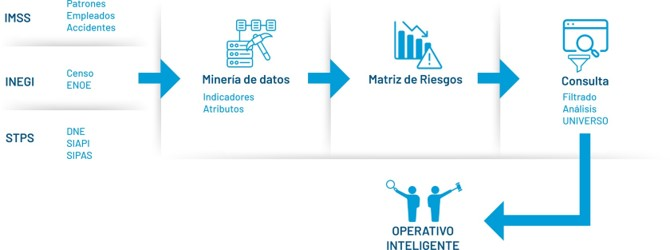
\includegraphics[width=0.5\linewidth]{images-1/01/esquemaPPTSalafranca} \caption{Presentación esquematizada de la solución}\label{fig:esquemaPPTSalafranca}
\end{figure}

\textbf{LA IMAGEN ANTERIOR REEMPLAZARÍA ESTA OTRA}

\begin{figure}
\centering
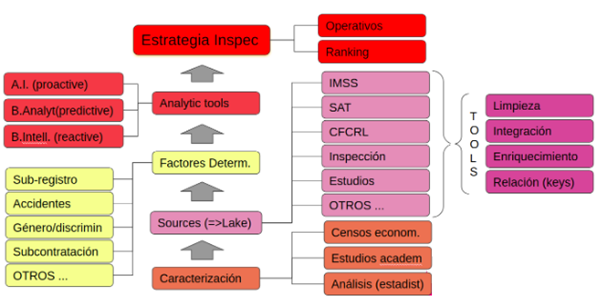
\includegraphics{images-1/01/Ilustracion1.png}
\caption{Ilustración XXX:}
\end{figure}

En el esquema anterior se puede observar los componentes básicos de la solución planteada, que tienen que ver con:

\begin{itemize}
\tightlist
\item
  \st{La concentración y procesamiento de la información estadística y los estudios especializados que permiten el análisis de las redes y cadenas productivas, del contexto laboral y su caracterización en materia de actividad económica, ocupación, empleo, evolución de los sueldos y salarios, etc.}
\item
  La limpieza, enriquecimiento y relacionamiento de información que se pudo integrar en bases de datos para su análisis. Esta información, como ya se mencionó, proviene tanto de fuentes internas como externas, a través de convenios de colaboración.
\item
  La determinación de los criterios de análisis que buscaron identificar las principales violaciones y que reflejen las prioridades en materia de política pública que deben guiar la inspección del trabajo.
\item
  El desarrollo de las herramientas que, a partir del establecimiento de los criterios mencionados y su descomposición en indicadores, permitieron llevar a cabo análisis basados en algoritmos de analítica, minería de datos y aprendizaje de máquina.
\end{itemize}

\hypertarget{introalcance}{%
\subsection{Alcance}\label{introalcance}}

El SIDIL tiene como alcance:

\begin{itemize}
\tightlist
\item
  Desarrollar una matriz de criterios sustantivos para la identificación de las principales violaciones laborales por parte de los patrones, desagregados en los indicadores necesarios y factibles para su evaluación en las empresas y centros a partir de las fuentes de información que se disponen.
\item
  A partir de un diagnóstico pormenorizado contar con la identificación de los acervos de información susceptibles de incorporarse, así como las necesidades de procesamiento que son necesarias para integrar estos datos al cálculo de los indicadores generados.
\item
  La implementación de un repositorio de información y un ambiente de analítica de datos con las bases de datos procesadas y listas para su incorporación.
\item
  Una serie de interfaces y servicios de información que permitan la consulta del repositorio de datos a través de los indicadores y criterios definidos para la generación de estrategias inteligentes para la inspección.
\item
  La transferencia del conocimiento y de las herramientas necesarias para asegurar la sostenibilidad del proyecto en el mediano plazo.
\end{itemize}

\hypertarget{estructura-y-flujos-de-trabajo-del-sidil}{%
\section{Estructura y flujos de trabajo del SIDIL}\label{estructura-y-flujos-de-trabajo-del-sidil}}

Esta sección describe a detalle y para una audiencia técnica los algoritmos computacionales, las fuentes de información y los metadatos que las caracterizan, para la tarea de lograr el cálculo de una predicción de riesgo de incumplimiento de la normatividad en materia laboral e imputarlos a los CT del Directorio Nacional de Empresas (DNE) de la STPS. Se ofrece información respecto a:

\begin{enumerate}
\def\labelenumi{\arabic{enumi})}
\item
  \textbf{El \emph{flujo de información}} establecido para el funcionamiento del SIDIL.
\item
  \textbf{El \emph{propósito} de} cada uno de los módulos, procesos y productos contenidos en el SIDIL.
\item
  \textbf{Las \emph{actividades}} que se deben realizar en cada uno de los módulos para mantener actualizado el SIDIL.
\end{enumerate}

La principal audiencia de este documento es el personal de la STPS, particularmente de la Dirección General de Investigación y Estadísticas del Trabajo (DGIET), la cual será responsable de mantener actualizado el SIDIL, particularmente en lo que respecta al procesamiento de datos para la producción de la Matriz de Predicción de Riesgo (MPR). De hecho, tanto el alcance del SIDIL, como el de este documento en general incorpora como un requisito la estrecha colaboración que se ha sostenido entre la Dirección de Estrategia e Innovación de AIR y la Dirección General de Investigación y Estadísticas del Trabajo (DGIET) de la STPS. Se han sostenido un gran número de sesiones de trabajo técnico y reuniones ejecutivas que, reflejando los intereses y capacidades de la STPS, dieron forma a la configuración actual del sistema.

La estructura de este apartado sigue en buena medida el diseño modularizado del SIDIL. Se presentan las cuestiones generales del sistema, haciéndolo en dos diferentes niveles: por un lado para una audiencia menos técnica se detallan algunos aspectos sustantivos comunes a los diferentes elementos del sistema; por otro lado se presentan aquellas especificaciones que, si bien más técnicas, tienen implicaciones para los diferentes módulos del sistema y que se enuncian sólo una vez en esta sección para evitar su repetición en los capítulos restantes del documento. Del mismo modo se presentan los módulos en los que suceden todos los procesos para mantener actualizada la predicción de riesgos en diferentes submaterias a un universo de naturaleza dinámica de centros de trabajo consultados del Directorio Nacional de Empresas (DNE). También se ofrecen detalles del diseño y operación de la interfaz de consulta, que constituye el módulo III y que, tomando la Matriz de predicción de Riesgos (MPR), resultado del proesamiento, permite a un usuario de la UTD, seleccionar a los CT con base en la predicción de riesgo por submaterias, atributos observados e indicadores imputados a todos los CT que se encuentran en el DNE. Finalmente se presenta el modelo predictivo utilizado, mismo que emana de combinar los hallazgos de todas las inspecciones laborales realizadas por la UTD con todos los indicadores laborales calculados de manera histórica, según la disponibilidad temporal de las fuentes de información.

\begin{figure}
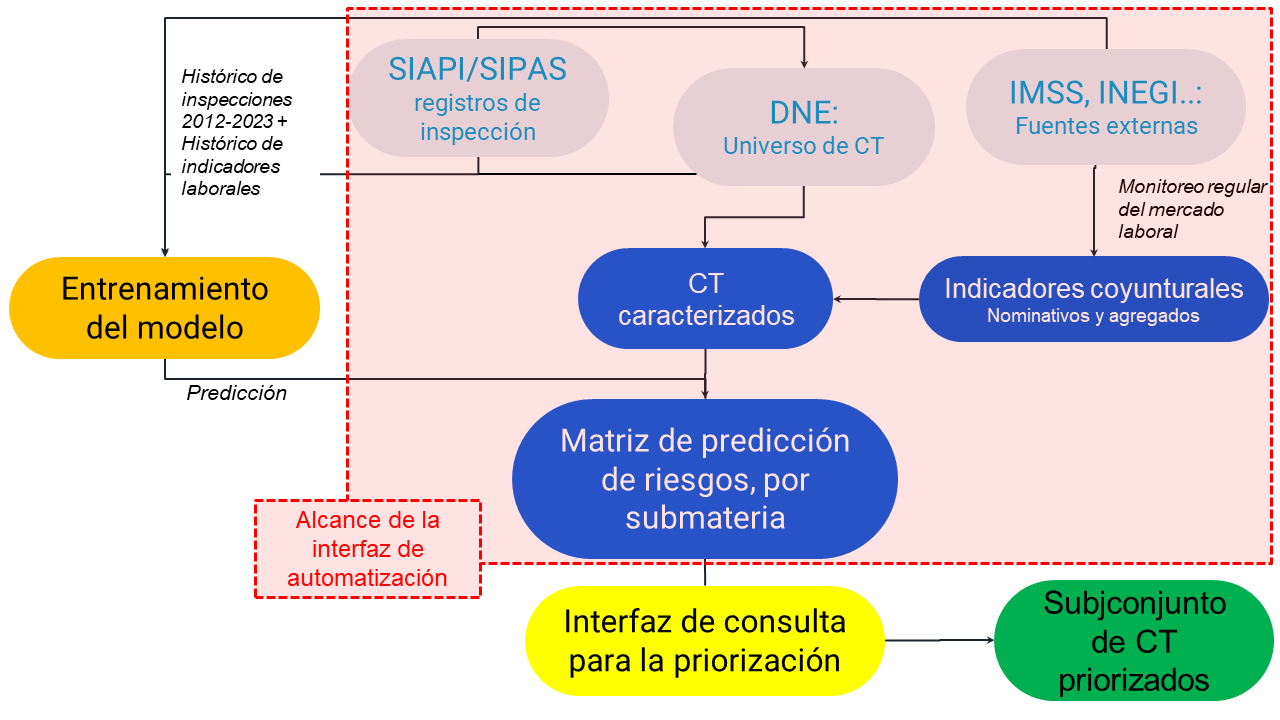
\includegraphics[width=0.5\linewidth]{images-1/02/image2_alternativaTD} \caption{Pipeline simplificado del SIDIL  (versión simplificada)}\label{fig:pipelsimplaaificado2}
\end{figure}

\hypertarget{elementos-buxe1sicos-del-sidil}{%
\subsection{Elementos básicos del SIDIL}\label{elementos-buxe1sicos-del-sidil}}

\textbf{El objetivo del SIDIL es construir una predicción de riesgo de incumplimiento a la normativa laboral vigente de los centros de trabajo de las empresas, a partir de la explotación de diferentes fuentes de información.} De esta manera, con esta predicción de riesgo y otros indicadores y atributos asociados a los centros de trabajo, se pueden construir universos con mayor probabilidad de incumplimiento en determinadas submaterias que forman parte del alcance normativo de las inspecciones laborales.

Para dicho objetivo, el SIDIL explota diferentes fuentes de información de una manera sistematizada. \textbf{El SIDIL se basa en un conjunto ordenado y sincronizado de algoritmos (s,cripts) que a partir de información contenida en archivos de entrada (inputs) crea otros archivos de salida (outputs)}, a partir de un proceso modularizado conectado.

\begin{figure}
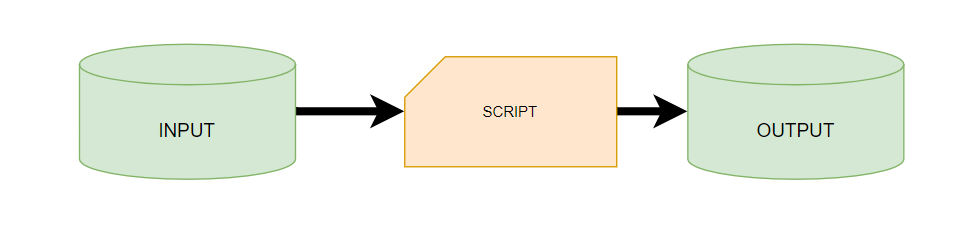
\includegraphics[width=0.5\linewidth]{images-1/02/script_input_output} \caption{Relación input-script-output}\label{fig:scriptinputoutput}
\end{figure}

Definamos los tres elementos presentados en la ilustración \ref{fig:scriptinputoutput}:

\textbf{Entradas o Inputs}: son tablas de información con campos y observaciones de interés para el SIDIL. Existen tres tipos de inputs.

\begin{itemize}
\item
  Inputs exógenos: fuente de información ``original'' o ``cruda'' no producida por el SIDIL, pero relevante para su funcionamiento. Por ejemplo, la Encuesta Nacional de Ocupación y Empleo del INEGI que se utiliza para la obtención de indicadores. También pueden ser registros administrativos como lo son el DNE de la propia STPS o el patrón de empleadores registrados ante el IMSS, entre otros.
\item
  Catálogos: dan sentido, facilitan el mantenimiento e interpretación, y homologan los campos presentados en otras fuentes de información. Por ejemplo, las etiquetas asociadas al marco geoestadístico de municipios y entidades del país, producido por INEGI.
\item
  Inputs que provienen de datos generados en una etapa anterior: por consistencia, el SIDIL, al procesar una fuente de información exógena, con o sin apoyarse en catálogos, genera outputs que, al ser parte de un sistema modularizado o compartimental, sirven de inputs para una siguiente etapa. Por ejemplo, el acervo de indicadores laborales generados a partir de la ENOE son un output del módulo I de actualización de indicadores - que sirve de input para el módulo de imputación de indicadores al universo de centros de trabajo, como se describirá más adelante.
\end{itemize}

\textbf{Scripts}: son documentos (textos) que contienen instrucciones para la ejecución de algoritmos de cómputo (secuencias de comandos) que instruyen a un procesador para cargar, transformar y generar información. Los scripts toman la información de los inputs y, mediante diversas operaciones transforman la información, generando outputs que servirán de insumo para etapas posteriores o como resultado final. En esencia los scripts conforman la médula espinal del SIDIL, toda vez que su contenido e interacción permite procesar la información de manera consistente a lo largo del tiempo. Existen varios tipos de scripts. Entre ellos hay algunos de carácter general y otros específicos para cada fuente de información. Los primeros se detallan en la sección 3.3, mientras que los segundos se profundizan en las secciones correspondientes de cada módulo.

\textbf{Salidas o Outputs}: Son resultado de aplicar uno o más scripts a una o más fuente de información o inputs. Contienen información considerada relevante, procesada, y estructurada para su interpretación humana o bien como un insumo para una próxima etapa en el SIDIL. Es decir, como referido anteriormente, un output de una etapa puede ser un input de otra etapa.

A partir de los tres elementos presentados anteriormente: inputs, scripts y outputs, queda claro que el SIDIL es un sistema de procesamiento de información que descansa sobre la coherencia y consistencia entre estos tres elementos.

\hypertarget{modulosqueconformanSIDIL}{%
\subsection{Módulos que conforman el SIDIL}\label{modulosqueconformanSIDIL}}

En esta sección se describen de manera general los propósitos y procesos que se realizan en cada uno de los módulos del SIDL, a fin de ofrecer una explicación de sus principales características.

Conviene enfatizar la importancia y motivación de tener un SIDIL compuesto por módulos diferenciados, ya que gracias a su modularidad el SIDIL es más sostenible, toda vez que aísla potenciales problemas en el procesamiento entre los diferentes módulos. Es decir, ante la eventual imposibilidad de correr un módulo, si bien puede implicar la no actualización de dicha información, no afecta la actualización de otros módulos.

A su vez, la compartimentalización se observa, cuando es posible, al interior mismo de los módulos. Por ejemplo, si hubiera un cambio en uno de los campos de una fuente de información que impidiera el cálculo de cierto indicador, esto no inhibe la actualización de otros indicadores de dicha fuente de información.

Así mismo, la modularización abona a la facilidad de dar mantenimiento a los diferentes componentes del SIDIL. La ejecución de los módulos por separado (en contraste con una ejecución única de todos los módulos) hace que, de presentarse problemas o de ser necesarias una revisión, ésta pueda concentrarse en los módulos en donde fuera de interés sin afectar a los demás módulos. La modularización permite aprovechar posibles ventajas comparativas, áreas de especialización e incluso atribuciones heterogéneas al interior de la STPS, permitiendo limitar el acceso a ciertas carpetas o subcarpetas en las que se alojan los inputs o scripts de ciertos módulos.

\begin{verbatim}
## [1] "aqui PIPELINE"
\end{verbatim}

El SIDIL tiene cuatro módulos, tal como se muestra en la ilustración \ref{fig:modulosSIDIL}: El \protect\hyperlink{moduloIexplicaciongeneral}{primer módulo} es el de actualización de indicadores, mismo que explota las fuentes de información exógenas; el \protect\hyperlink{moduloIIexplicaciongeneral}{segundo módulo} es el de consulta al universo de CT registrados en el DNE, la imputación de indicadores y de predicción de riesgo, que incorpora los resultados del módulo anterior. Estos dos módulos son operables a través de una \protect\hyperlink{moduloIyIIexplicaciongeneral}{interfaz de automatización}, misma que a su vez permite de una manera muy simple, asegurando coherencia y consistencia, la incorporación y actualización de catálogos y fuentes de información.

Así, la interfaz de automatización abarca el desarrollo de los procesos que están en color azul en esta ilustración. Luego, el tercer módulo es el de la \protect\hyperlink{interfazConsultaexplicaciongeneral}{interfaz de consulta}, que explota el principal resultado del módulo anterior (la Matriz de Predicción de Riesgos, MPR). Esta consulta está esquematizada en el área verde de la figura, y da como resultado un \emph{listado de centros de trabajo priorizados}, listos para ser incorporados a la programación de inspecciones. Por último, el cuarto módulo, de entrenamiento, es el que permite reentrenar el modelo para actualizar la forma en la que se realizará la predicción. El módulo cuarto arroja un modelo predictivo entrenado (llamémoslo ``parámetros del modelo'') que el módulo II consulta para la predicción del modelo sobre el universo de CT enriquecido con los indicadores. A continuación, se ofrecen las principales características de estos módulos.

\begin{figure}
\includegraphics[width=50px,style="float:left; background-color: #f5f5f5; padding-right:1em"]{images-1/important-icon} \caption{Modularización del SIDIL}\label{fig:modularizacionSIDIL}
\end{figure}

\begin{rmdcomment}
El SIDIL está compuesto por diferentes módulos. Adicional a las ventajas
mencionadas, conviene enfatizar que el SIDIL permite a los usuarios
actualizar los diferentes módulos por separado. Esto es, diferentes
usuarios (supongamos, especializados por fuentes de información) pueden,
en distintos momentos del tiempo, actualizar un módulo sin necesidad de
realizar la actualización de los demás módulos en el mismo momento.
Esto, si bien no se reflejará en una actualización de la matriz de
predicción de riesgos a menos que se actualice el módulo II, permite
dividir las tareas entre diferentes personas.

En ese sentido, una situación que podría ocurrir es la siguiente: el
módulo I se actualiza cada tres meses. Pero en el caso del módulo II, al
depender del universo de CT registrado en el DNE, puede ameritar
actualizarse con mayor frecuencia, toda vez que dicho registro
administrativo está en constante cambio (nuevos CT que se incorporan o
modificaciones que se realizan a CT preexistentes). No es necesario (ni
abonaría nuevos indicadores) volver a correr el módulo I porque el DNE
haya sufrido cambios. La información sería la misma.

De la misma manera, la modularización permite aislar la tarea más
compleja del SIDIL: la actualización del módulo IV de entrenamiento del
modelo. Esta tarea es la más intensiva en tiempo, toma de decisiones y
acceso a información a la vez que, de mantenerse el mismo modelo, no
resultaría en sustantivas diferencias si la actualización se realizara
con elevada frecuencia.
\end{rmdcomment}

\hypertarget{moduloIexplicaciongeneral}{%
\subsubsection*{Módulo I: actualización de indicadores}\label{moduloIexplicaciongeneral}}
\addcontentsline{toc}{subsubsection}{Módulo I: actualización de indicadores}

En este módulo se explotan las diversas fuentes de información que sirven como input. \textbf{El objetivo de este módulo es poder medir fenómenos laborales a través de indicadores que permiten caracterizar las condiciones vigentes en los centros de trabajo.} Para tal fin los scripts extraen y transforman los inputs para mantener actualizados dichos indicadores. Es en este módulo en donde, a futuro, es posible agregar o quitar indicadores laborales según surjan nuevas fuentes de información o entren en desuso otras.

Todas las estimaciones puntuales (valores) de los indicadores se calculan para diferentes ``niveles de agregación'': \emph{\textbf{entiéndase por nivel de agregación aquella combinación de campos de tamaño del centro de trabajo, clasificación industrial y ubicación geográfica que caracterizan a cada centro de trabajo.} Hay 18 niveles de agregación según se incorporen estos campos. A mayor combinación de campos y/o especificidad en la utilización de los mismos, mayor es el nivel de agregación y más específica es la estimación puntual. Para más información consultar la sección 4.1.3.1 de este documento.}

\begin{figure}
\includegraphics[width=50px,style="float:left; background-color: #f5f5f5; padding-right:1em"]{images-1/important-icon} \caption{El aprovechamiento de los niveles de agregación en el cálculo de indicadores.}\label{fig:utilidadestimacionespuntuales}
\end{figure}

\begin{rmdcomment}
Sirve dar un ejemplo de la utilidad de calcular las estimaciones
puntuales de los indicadores a diferentes niveles de agregación: Para el
cálculo de la media de la tasa de prevalencia de asalariados percibiendo
hasta 105\% del salario mínimo (uno de los indicadores desarrollados) a
nivel nacional, el promedio asciende a 12.8\% de los puestos asegurados.
Esto significa que casi 13\% de los asegurados en el IMSS perciben hasta
105\% del salario mínimo. Este es el promedio nacional y es el nivel de
agregación de menor granularidad o especificidad. Pero detrás de este
promedio hay una elevada heterogeneidad: tan solo observando el
siguiente nivel de agregación que distingue por categoría de tamaño se
percibe que los centros de trabajo (CT) de hasta 10 personas aseguradas
tienen una prevalencia del 21.7\%, mientras que las de 251 o más
asegurados se reduce a 0.77\%. Si además a los CT de menor tamaño se les
distingue por la clasificación industrial a dos dígitos, se estima que
aquellas en la categoría industrial SCIAN: 11 (Agricultura, cría y
explotación de animales) tienen un promedio de 21.3\% pero las SCIAN 21
(minería) un promedio de 16.9\%. Este último nivel de agregación ya
recupera la información de dos campos (tamaño y clasificación industrial
a dos dígitos), pero puede profundizarse aún más incorporando la
dimensión geográfica (entidad federativa y municipio) y además llevar a
3 dígitos la clasificación industrial. De esta manera, a mayor
incorporación de dimensiones, o mientras más específicas sean éstas más
preciso es el dato. A mayor precisión, mayor la posible heterogeneidad
en la caracterización de los CT y mayor poder predictivo de los
indicadores (sobre este punto se ofrecen más detalles en la sección 6).
\end{rmdcomment}

El cálculo de un determinado indicador se realiza para cada uno de los diferentes niveles de agregación. Esto para permitir que a un CT se le pueda imputar una mejor estimación de riesgo si se conoce con mayor detalle sus características de tamaño, industria y geografía, pero que, en caso de ausencia de alguna de ellas se le atribuya una medida de una agrupación más general. Esto permite aprovechar al máximo la información disponible.

Esto significa que, si la estructura de información del input lo permite, la información se explota al máximo nivel de granularidad y cobertura posible. En concreto, y para poner un ejemplo: de la ENOE se calcula la tasa de sindicalización (con el cuestionario ampliado del primer trimestre de cada año) para todas las posibles combinaciones de entidad federativa, clasificación industrial a dos y tres dígitos del SCIAN y categorías de tamaño, independientemente de que para ciertas combinaciones de estos tres campos no hubiera CT que ``requieran'' dicha caracterización. Es decir, podría ser el caso de que se calcule para la categoría industrial 111 en la entidad federativa 1 y categoría de tamaño 1 dicho indicador, incluso aunque, por diferentes motivos, el DNE no tenga a ningún CT con dichas características.\^{}{[}De manera análoga, dado que el SIDIL explota registros administrativos del IMSS y calcula ciertos indicadores a nivel \emph{registro} patronal, cabe observar que los indicadores se calculan para todos los registros patronales, independientemente de que éstos sean ``encontrados'' en el DNE.{]} De esta manera, dada la posibilidad de que en cualquier momento se incorporen nuevos CT al DNE con esta o cualquier otra combinación de información, se tiene a disposición la información en todos los niveles de agregación para su eventual aprovech

\begin{figure}
\includegraphics[width=50px,style="float:left; background-color: #f5f5f5; padding-right:1em"]{images-1/important-icon} \caption{El aprovechamiento de los niveles de agregación en el cálculo de indicadores (segunda parte)}\label{fig:aprovechamientonivelesagregacion}
\end{figure}

\begin{rmdcomment}
Con lo mencionado sobre el módulo de actualización de indicadores se
permite anticipar los elementos más importantes en la estrategia y
operacionalización del ``matching'' o imputación de indicadores
laborales al universo de centros de trabajo (que se informa a mayor
detalle en el capítulo 4.2.5): el acervo de estimaciones puntuales (por
ejemplo la media de acceso a la seguridad social) calculada para toda la
combinación posible de tamaño, clasificación industrial y ubicación
geográfica, es imputado a los CT a partir de un algoritmo que identifica
el nivel de especificación a lo largo de estos tres campos. Es decir, el
algoritmo detecta el nivel de agregación de cada uno de los CT y le
imputa la estimación puntual más granular o específica posible de
acuerdo con la información disponible de cada CT. ¿Cuál es la ``más
granular o especifica posible''? Es aquella estimación puntual que
incorpora la mayor cantidad de campos de tamaño, clasificación
industrial y geografía posible.
\end{rmdcomment}

Además de que todas las estimaciones puntuales se calculan por niveles de agregación, cuando se trata de estimaciones puntuales de indicadores que explotan la fuente información IMSS, previo a su ``agregación'', se realiza su cálculo también por registro patronal. Esta información sirve para, como se describe en el módulo siguiente, imputar la información de \emph{manera nominativa} por registro patronal, siempre que el CT estuviera disponible (identificable) en el DNE.

\textbf{Los indicadores se expresan en el mismo sentido ordinal, donde ``más es mejor'', a excepción de cuando se encuentran en la MPR, como se verá más adelante:} todos los indicadores miden un fenómeno laboral que inherentemente reflejan una violación a un derecho laboral, o en última instancia, un juicio de valor. A menor valor absoluto de un indicador, mayor incumplimiento al derecho laboral, o en peores condiciones (de eso que se mide) están las personas trabajadoras. Por ejemplo, el acceso a la seguridad social cercano a 100\% indica una elevada tasa de formalización de la relación laboral, mientras que cercano a 0\% se acerca a la informalidad absoluta.

\textbf{En la construcción de la MPR (siguiente módulo), y a efectos de darle el mismo sentido que la predicción de la probabilidad de incumplimiento con la normativa laboral, el sentido de los indicadores se invierte.} Es decir, los indicadores que hasta ese momento expresan ``más es mejor'' se invierten para reflejar que ``más es peor''. Esto facilita la interpretación y el uso de los mismos como variables de selección y filtrado a la hora de explotar la MPR en la interfaz de priorización. De esta manera, al filtrar, tanto los predictores de riesgo generados a partir del modelo entrenado, como los indicadores calculados a partir de las fuentes de datos tienen la lógica de que un valor más cercano a 1 representa un mayor riesgo de violaciones.

\begin{figure}
\includegraphics[width=50px,style="float:left; background-color: #f5f5f5; padding-right:1em"]{images-1/important-icon} \caption{El sentido de los indicadores}\label{fig:sentidoindicadores}
\end{figure}

\begin{rmdcomment}
Todos los indicadores se expresan en el mismo sentido, en donde un menor
valor de un indicador se asocia a peores condiciones laborales en el
aspecto que se esté midiendo. Esto es importante porque en algunas
ocasiones (ver siguiente capítulo) algunos indicadores se expresan como
la inversa o el complemento (según se traten de tasas o no) de la
ocurrencia de un fenómeno laboral. Esto no guarda relación con la
estandarización de 0 a 1 y la inversión (es decir, el cambio de sentido)
de los valores imputados a los centros de trabajo registrados en DNE,
mismo que se realiza únicamente posterior a la imputación y sobre el
universo acotado y que permite ordenar en percentiles a los centros de
trabajo, siendo los percentiles de \emph{menor} valor aquellos que se
asocian a \emph{mejores} condiciones laborales (dada la estandarización
y posterior inversión).
\end{rmdcomment}

\textbf{En este módulo también se mantiene actualizada una base que registra la información más básica de los patrones registrados ante el IMSS, a efectos del enriquecimiento de la consulta del DNE (ver siguiente módulo).} Esto es adicional al acervo de estimaciones puntuales por registro patronal que se mencionó en el párrafo anterior.

En acuerdo con la DGIET, \textbf{se propone que este módulo se actualice cada tres meses}, toda vez que es la frecuencia con la cual se actualiza uno de los principales insumos (la ENOE del INEGI). Pero dado que los inputs del IMSS se actualizan mensualmente (y se calcula un promedio móvil de los últimos tres meses disponibles) tendría sentido hacerlo hasta una vez por mes si se desea.

\textbf{Así, el módulo I constituye la \ul{oferta} de estimaciones puntuales de los indicadores del SIDIL}, que posteriormente serán imputados (de manera nominativa o por nivel de agregación, según sea al caso) a los centros de trabajo disponibles en el DNE.

\hypertarget{moduloIIexplicaciongeneral}{%
\subsubsection*{Módulo II: Consulta al universo de CT, imputación de indicadores y predicción de riesgo}\label{moduloIIexplicaciongeneral}}
\addcontentsline{toc}{subsubsection}{Módulo II: Consulta al universo de CT, imputación de indicadores y predicción de riesgo}

En este módulo se consulta el Directorio Nacional de Empresas (DNE) para obtener el universo actualizado de centros de trabajo susceptibles de ser inspeccionados. En esta consulta los campos más importantes (además del identificador único del CT) son el tamaño, la clasificación industrial, el municipio y la entidad federativa del CT, a efectos de posteriormente poder imputarle los indicadores obtenidos del módulo anterior. Del mismo modo se obtienen campos adicionales considerados atributos y que pueden servir para, a través de la interfaz de consulta filtrar el universo de centros de trabajo. Un ejemplo de ello es el campo que indica que el CT forma parte de un mecanismo de autorregulación, como por ejemplo el Programa de Autogestión en Seguridad y Salud en el Trabajo -- un aspecto que se toma como dato del DNE.

\textbf{Si el módulo I constituye la ``oferta'' de indicadores, el módulo II, particularmente el universo de CT registrados en el DNE, representa la ``demanda'' de los mismos}. Son las características de los CT en el DNE las que determinan cuáles estimaciones puntuales de cada indicador serán imputadas a cada CT, notando que, en última instancia, de no poder caracterizar a un CT en ninguna de las tres dimensiones (clasificación industrial, geografía o tamaño) se le asignará el promedio a nivel nacional. Siguiendo con la analogía, la oferta y la demanda se encuentran justo en el punto que determina el algoritmo de matching coyuntural, es decir, la imputación de las estimaciones a los CT.

Como se menciona en la sección anterior, en aquellos campos de las tres dimensiones (geografía, tamaño e industria) el SIDIL consulta la información más actualizada disponible en el IMSS para que, en caso de que no estuviera el dato disponible en el DNE, se les impute dicha información (a efectos del SIDIL únicamente, no se modifican registros en el DNE, sino solamente en el resultado de la consulta a dicho directorio que utiliza el SIDIL). Esto permite ``refinar'' el nivel de agregación al que potencialmente se le imputan las estimaciones puntuales de los diversos indicadores a los CT. Por ejemplo, un CT puede no tener registrado el número de trabajadores en el DNE, en consecuencia, no sería posible tomar en consideración los niveles de agregación que requiere la estimación puntual por categoría de tamaño. Sin embargo, gracias a este procedimiento de enriquecimiento, si a través del registro patronal es posible identificar a este CT en las bases del IMSS, se le asigna el campo tamaño (contando el número de trabajadores registrados en el mismo) para imputarle una estimación puntual con el mayor nivel de agregación posible que incluya el tamaño como dimensión. Asimismo, a partir de esta identificación univoca de los CT en las bases del IMSS y del DNE, se realiza la imputación nominativa de los indicadores del IMSS.

Además, el SIDIL prevé una consulta al SIAPI y al SIPAS en caso de que la información contenida en el DNE no estuviera completa o estuviera actualizada. Dado que el SIAPI y SIPAS están en un proceso de desarrollo, por ahora este aspecto no se enfatiza en el manual. Pero un ejemplo de esta información podría ser el cálculo del porcentaje de inspecciones a un CT que terminaron en negativas patronales, en caso de que esto fuera de interés para la STPS para explotar en la interfaz.

\hl{AQU POSIBLEMENTE CONVIENE INCORPORAR UNA ILUSTRACION SOBRE RELACION SIAPI SIPAS, DNE Y SIDIL}

\begin{figure}
\includegraphics[width=50px,style="float:left; background-color: #f5f5f5; padding-right:1em"]{images-1/important-icon} \caption{Relación DNE-SNILE-SIAPI-SIPAS con el matching nominativo del IMSS}\label{fig:relacionDNESNILESIAPISIPAS}
\end{figure}

\begin{rmdcomment}
Actualmente el SIDIL consulta al DNE y al SIAPI/SIPAS. Al realizarlo, se
encuentra que en el DNE el campo número de trabajadores tiene
aproximadamente un 80\% de observaciones nulas (sin valor válido). Este
campo es enriquecido con el campo que se completa durante en las
inspecciones registradas en SIAPI SIPAS. Si es posible enriquecerlo
entonces ese campo ya se considera completo y no se realiza la
imputación de enriquecimiento con base en el IMSS patronal. Si en cambio
no hay un dato derivado de las inspecciones, entonces sí se busca el
enriquecimiento con los datos del IMSS. Por supuesto, se reconocen
obvias limitaciones derivadas de que en el IMSS se registra únicamente
el empleo formal mientras que en las inspecciones se registra todo tipo
de trabajadores, estén o no registrados ante el IMSS.
\end{rmdcomment}

En resumen, el proceso de imputación o ``matching'' tiene tres etapas, en dos scripts diferentes:

\begin{itemize}
\item
  Primero, se busca enriquecer aquellos campos que definen el nivel de agregación al que se le imputarán los indicadores. Esto es, que se complemente un campo vacío del DNE respecto al tamaño, geografía y/o clasificación industrial con la información disponible en las bases del IMSS (siempre y cuando se logre identificar al mismo CT en el DNE y en el IMSS). Esta primera etapa sucede inmediatamente posterior a la consulta del DNE, como parte de dicho script; mientras las siguientes dos etapas suceden en el script de matching coyuntural.
\item
  Segundo, se le imputan indicadores de manera nominativa, cuando aplique y siempre que fuera posible, a través del campo registro patronal, identificar a un CT del DNE en las bases del IMSS. A esto se le llama \emph{imputación nominativa}.
\item
  Tercero, para todos los CT y todos los indicadores a los que no fue posible realizarle una imputación nominativa, se le imputa un valor de todos los indicadores por nivel de \emph{agregación} según la información disponible de cada CT.
\end{itemize}

Hasta aquí se obtiene el universo de los CT extraído del DNE y enriquecido con las estimaciones puntuales de todos los indicadores disponibles.

\textbf{A partir de los indicadores imputados a cada uno de los CT, y con base en el modelo entrenado (ver módulo IV) se calculará el riesgo de incumplimiento de cada uno de ellos por submateria.} La información de indicadores, para cada uno de los CT del universo, se utiliza como insumo para el cálculo de factores que permitirán la predicción del riesgo de incumplimiento en cada una de las submaterias de las Condiciones Generales de Trabajo a través de la \textbf{aplicación del modelo} (previamente entrenado\^{}{[}Conviene enfatizar que no es en este módulo donde se entrena el modelo, ya que eso forma parte del módulo IV, en este caso sólo se aplica el modelo previamente entrenado.) para predecir y atribuir un factor de riesgo de incumplimiento a cada centro de trabajo para cada submateria.

El resultado final de este módulo es la \textbf{Matriz de Predicción de Riesgos} (MPR), misma que se analiza en mucho más detalle en la sección. 3.10. Aquí conviene mencionar que la MPR tiene tantas filas como centros de trabajo registrados en el DNE y el número de columnas dependerá de la disponibilidad de indicadores, del número de atributos que se consulten al DNE (cuando menos serán aquellos campos de geografía, clasificación industrial y tamaño) y del número de submaterias sobre las cuales se realiza una predicción de riesgo, como muestra la Ilustración 3 a continuación.

\begin{figure}
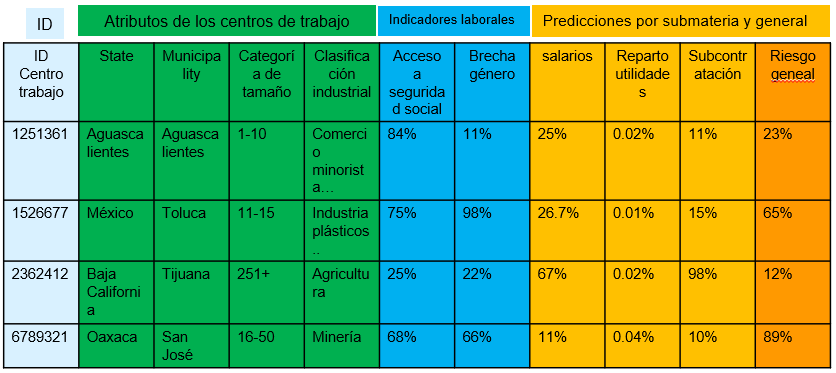
\includegraphics[width=11.61in]{images-1/02/MPR_simplificada} \caption{Matriz de predicción de riesgos (ilustración simplificada)}\label{fig:MPRsimplificada}
\end{figure}

\hypertarget{moduloIyIIexplicaciongeneral}{%
\subsubsection*{Módulos I y II: operables desde la interfaz de automatización}\label{moduloIyIIexplicaciongeneral}}
\addcontentsline{toc}{subsubsection}{Módulos I y II: operables desde la interfaz de automatización}

\textbf{La interfaz de automatización permite que, bajo circunstancias normales, es decir, sin la necesidad de corregir los algoritmos de cálculo, se puedan mantener actualizados los productos de los módulos I y II sin necesidad de ejecutar los algoritmos desde la consola del software de análisis R Studio}, sino desde una interfaz amigable y simplificada que ejecuta los mismos procesos que se correrían manualmente desde R Studio. A dicha interfaz también se le agregó la funcionalidad de incorporar actualizaciones a las fuentes de información (por ejemplo, un nuevo trimestre de la ENOE) o a los catálogos que permiten la adecuada explotación de los insumos a través de parámetros configurables. Esto permite que la interfaz mantenga actualizados los productos módulos I y II, y que esto se realice, en circunstancias normales, por personal que no requiere de acceso o conocimiento profundo de un software especializado. La interfaz permite actualizar los insumos del cálculo, modificar sus parámetros principales y seleccionar cuáles procesos se quieren ejecutar a fines de actualizar los productos, todo el tiempo reportando en una consola los principales avances de dichos procesos, para seguimiento del usuario que lo ejecuta.

\textbf{En el proceso de la actualización de los módulos I y II desde esta interfaz, en la consola de procesamiento se presenta solamente la información más ejecutiva sin abundar en todo el detalle técnico del procesamiento de información.} Esto implica, que: a) la interfaz permite la ejecución automatizada de los códigos del módulo I y II, más no exime de la responsabilidad de analizar los resultados reportados en su consola; y b) la interfaz no presenta toda la información que un usuario más técnico pudiera requerir para su análisis y comprensión de los procedimientos ejecutados, la que se encuentran en las bitácoras de cada proceso, también accesibles para un usuario más avanzado. Por último, realizadas las principales actualizaciones, la interfaz permite la descarga de la MPR más reciente y enviarla a la interfaz de consulta, poniendo así la MPR a disposición del otro tipo de usuario del SIDIL, el personal de la UTD, para la priorización de CT conforme a las estrategias de selección que se presenten.

\textbf{En contraste con la interfaz de consulta (ver más adelante), esta interfaz, si bien facilita la ejecución de los módulos I y II, sí requiere de cierto conocimiento técnico} -- estadístico en cuanto a que algunos de los mensajes que se reportan en su consola, si bien sólo se reportan a título informativo y no se espera una aprobación explícita del usuario, permiten a un usuario informado determinar que los resultados obtenidos guardan sentido. Por ejemplo, en un momento determinado la actualización de los indicadores del IMSS reporta el porcentaje que las mujeres representan en el total de personas aseguradas. Un usuario informado sabe que aproximadamente este porcentaje se ubica alrededor del 40\% y que cualquier desviación sustantiva de dicho porcentaje pudiera implicar que la identificación del sexo a partir de la CURP de las personas aseguradas no resultó satisfactoria o que hubo algún problema en el procesamiento realizado. De manera análoga, un usuario experimentado conoce el total de personas ocupadas que se estiman a partir de la ENOE (y sabe cómo validar esta estimación en el portal del INEGI), por lo que cualquier desviación sustantiva de una estimación normal tendría que llamarle la atención, ameritar la interrupción del proceso e iniciar una revisión exhaustiva a nivel código para encontrar la solución a dicho error de cálculo.

Recuadro 6:

\begin{figure}
\includegraphics[width=50px,style="float:left; background-color: #f5f5f5; padding-right:1em"]{images-1/important-icon} \caption{La utilización de la interfaz de automatización}\label{fig:utilizacioninterfazauto}
\end{figure}

\begin{rmdcomment}
La interfaz de automatización permite a un usuario mantener actualizados
los productos de los módulos I y II sin necesidad de ejecutar los
algoritmos desde la consola del software R. De hecho, no requiere tener
instalado el software R ni R Studio localmente, toda vez que la
operación de dicha interfaz se realiza desde una conexión WEB a un
servidor. Algunas de las condiciones que deben darse para que la
actualización de estos módulos desde la interfaz sea satisfactoria son:

\begin{enumerate}
\def\labelenumi{\arabic{enumi})}
\item
  Que no haya cambios sustantivos en los insumos de las fuentes de
  información o que no pudieran ser atendibles con la actualización de
  catálogos. Por ejemplo, hay un catálogo de campos que permite asociar
  diferentes nombres de ciertas variables a un nombre único, para
  atender a cambios menores entre algunas versiones de la misma fuente
  de información. Este tipo de cambios se considera menor y es atendible
  desde el catálogo.
\item
  Que se requieran incorporar nuevos indicadores, o actualizar el método
  de cálculo de algunos indicadores, o incluso modificar el flujo de
  información. En otras palabras, cualquier modificación al cómo se
  procesa la información, implica que primero haya que modificar algunos
  archivos a nivel ``código'' y esto no se puede realizar desde la
  interfaz.
\item
  Que se opte por utilizar un modelo entrenado distinto al más reciente.
  El SIDIL está configurado para utilizar la última versión del modelo
  entrenado. Si se quisiera, a fines comparativos, realizar una
  predicción con otro modelo, distinto al más reciente, entonces esto no
  podrá ser realizado desde la interfaz.
\end{enumerate}

En otras palabras, la interfaz de automatización permite mantener
actualizado los productos de los módulos I y II con un esfuerzo menor
que el requerido para abrir y ejecutar el código en una consola.
\end{rmdcomment}

\hypertarget{muxf3dulo-iii-consulta-de-la-mpr-para-priorizaciuxf3n-de-ct-a-inspeccionar}{%
\subsubsection{Módulo III: Consulta de la MPR para priorización de CT a inspeccionar}\label{muxf3dulo-iii-consulta-de-la-mpr-para-priorizaciuxf3n-de-ct-a-inspeccionar}}

En el módulo de consulta se explota la información contenida en la Matriz de Predicción de Riesgo (MPR). Se realiza a través de una interfaz interactiva, permitiendo al usuario escoger y ponderar diferentes campos para acotar y priorizar el universo de CT disponible en el DNE para logar un subconjunto de ellos que cumplen determinados criterios. Los CT en dicho subconjunto cumplen con características que reflejan la estrategia de inspección que se quiere desarrollar. Típicamente constituirán este subconjunto aquellos CT de mayor probabilidad de incumplimiento en cierta submateria y que además cumplen con los criterios impuestos a otras variables que los caracterizan.

\textbf{La utilización de esta interfaz no requiere conocimientos avanzados de estadística ni de econometría}: si bien el SIDIL es un proceso intensivo en datos, su producto final, la MPR, es explotado por el área de programación de las inspecciones a través de una interfaz amigable que permite reflejar prioridades estratégicas propias del proceso de planeación, particularmente aquellas que se dan en el marco de operativos de un alcance específico.

La interfaz permite al usuario:

\begin{enumerate}
\def\labelenumi{\arabic{enumi})}
\item
  Siempre utilizar la MPR más reciente. De manera predeterminada se carga la MPR de versión más reciente, motivado en que ésta refleja los insumos más recientes (que a su vez se generaron con las versiones más reciente de los diferentes insumos de información).
\item
  Escoger una submateria sobre la cual se realizó una predicción confiable (todos los CT tienen una predicción realizada en cada una de las submaterias, por lo que escoger cuál de ellas se utilizará para la programación de inspecciones no limita el número de CT). Una vez seleccionada la submateria, es posible acotar el universo limitándolo a aquellos CT que, para la predicción escogida, están en un rango numérico acotado (el rango de probabilidad).
\item
  Acotar el universo de CT a partir de la aplicación de filtros adicionales, a partir del resto de la información contenida en la MPR:

  \begin{enumerate}
  \def\labelenumii{\alph{enumii}.}
  \item
    Atributos de los CT obtenidos del DNE (por ejemplo, una entidad federativa) o enriquecidos a través del SIAPI SIPAS (por ejemplo, historial reciente de negativas patronales), o enriquecidos con el IMSS (por ejemplo, tamaño del CT).
  \item
    Indicadores calculados a partir de las diferentes fuentes de información. En esencia, todos aquellos calculados en el módulo I y asignados a los CT a partir de los primeros dos pasos del módulo II.
  \end{enumerate}
\end{enumerate}

\ul{\textbf{Módulo IV: Entrenamiento del modelo}}

Este módulo tiene como propósito entrenar el modelo predictivo para actualizar sus valores y posteriormente aplicarlos a la predicción que se realiza sobre el universo de CT enriquecido con indicadores coyunturales. A tal fin, en este módulo se realiza la explotación histórica de todas las fuentes de información.

\textbf{A diferencia del módulo de actualización de indicadores que explota el último periodo de referencia disponible para cada fuente de información, en este módulo se explotan todos los periodos de referencia disponibles para todas las mismas fuentes de información, incorporando, además, los resultados de todas las inspecciones realizadas a la fecha.} El SIDIL contempla que la explotación histórica de todos los indicadores laborales se realice desde 2012 en adelante, siempre que esté disponible la fuente de información. En concreto, dada la información disponible, estos son los periodos temporales cubiertos por fuente de información:

\begin{itemize}
\item
  ENOE: 2012 en adelante, de manera anual, utilizando el primer trimestre, toda vez que refleja la aplicación el cuestionario ampliado (ver sección 4.1.4.1.1).
\item
  IMSS: 2019 en adelante, de manera mensual, utilizando todos los meses (ver sección 4.1.4.2).
\item
  Censo Económico: 2019, toda vez que no preexiste un ejercicio similar al que realizó la STPS con el INEGI (ver más adelante sección 4.1.4.3).
\end{itemize}

\textbf{De esa manera, la explotación histórica no es otra cosa que repetir de manera iterativa el mismo procedimiento de generación de indicadores del módulo I pero extendiendo el horizonte temporal.} Claro está que conforme se extiende el periodo de referencia, aumenta el número de desafíos en materia de la infraestructura de cómputo y estructura de datos. Por poner un ejemplo, varios campos de columnas en insumos del IMSS cambian de nombre a lo largo del tiempo (motivo por el cual se estableció un catálogo de campos que permite armonizar dichos campos).

\textbf{La diferencia sustantiva entre el módulo II y el módulo IV, además de la extensión del periodo temporal para el cálculo de indicadores, es que, a diferencia del módulo II, en el módulo IV la unidad de observación no es el centro de trabajo sino la inspección a nivel submateria.} Para predecir la probabilidad de incumplimiento a cada uno de los CT en el entrenamiento del modelo se incluye en el análisis el universo de de 1.1 millones de inspecciones, que genera más de 5.8 millones de pares inspecciones--submaterias distintas.

La explotación histórica de todas las fuentes de información, inclusive los resultados de las inspecciones, permite la \textbf{interacción entre variables} provenientes de diferentes fuentes en el entrenamiento del modelo de aprendizaje de máquina (machine learning) que se utiliza para la predicción de riesgo. El modelo utilizado para este fin es el \textbf{Random Forest}, dadas que las pruebas realizadas con la información provista por la STPS dieron mejores resultados de predictibilidad con este modelo. Sin embargo, esto puede y debe revisarse conforme avance la literatura y la tecnología en esta materia.

Un \textbf{modelo Random Forest (RF) de aprendizaje automático utiliza múltiples árboles de decisión para hacer predicciones sobre un conjunto de datos}. Los árboles de decisión son un tipo de modelo de aprendizaje automático que se utiliza para tomar decisiones basadas en datos. Se representan gráficamente como un árbol, donde cada nodo representa una decisión o una acción (en este caso, una variable atributo o indicador asociado a los CT) y las ramas que se desprenden de él representan las posibles opciones que se pueden tomar.

\textbf{En el caso del modelo de RF que se utiliza, cada árbol de decisión en el modelo es una representación gráfica de las reglas que se utilizan para predecir la probabilidad de incumplimiento en una de las submaterias de inspección}. Cada árbol en el modelo toma como entrada los indicadores que se han calculado para el centro de trabajo que se está evaluando y, a través de una serie de preguntas, clasifica el centro de trabajo en una de las dos categorías: violación o no violación procedente en la submateria en cuestión.

\hl{Placeholder imagen pixelada pendiente mejora}

\begin{figure}
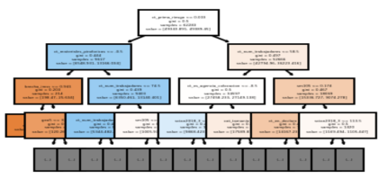
\includegraphics[width=5.26in]{images-1/02/arbol_decision} \caption{Ejemplo de un árbol de decisión}\label{fig:arboldecision}
\end{figure}

\textbf{En lugar de utilizar un solo árbol de decisión, el modelo RF utiliza múltiples árboles de decisión para mejorar la precisión de las predicciones.} Cada árbol se entrena con diferentes subconjuntos de los datos y se combinan las predicciones de todos los árboles para determinar la probabilidad de incumplimiento del centro de trabajo en cada área de inspección.

\textbf{En este caso, el RF se utiliza como ``multioutput'', es decir, para predecir la probabilidad de que un CT incumpla en cada una de las submaterias de inspección laboral, independientemente de la probabilidad de incumplimiento en otras submaterias.} El modelo funciona al tomar en cuenta los indicadores imputados a los centros de trabajo y analizar cómo se relacionan con el historial de incumplimiento en diferentes áreas de inspección. Luego, utiliza esta información para hacer una predicción sobre la probabilidad de que un CT incumpla en el futuro. Esto lo hace para cada una de las submaterias, de manera independiente.

\textbf{El número de observaciones que entra en el entrenamiento del modelo equivale al número de inspecciones a nivel submateria para las cuales hubo un desahogo registrado en el sistema.} Es decir, un centro de trabajo con un ID determinado, pudo haber sido inspeccionado en más de un año diferente. En cada una de esas inspecciones, se pudieron haber cubierto las mismas o diferentes submaterias. Por cada combinación de estos factores (ID del centro de trabajo, de la inspección y de la submateria), habrá una fila en la base que se conforma para el entrenamiento. Para un mismo CT y año, aunque fueran diferentes submaterias, los valores de los indicadores imputados de manera nominativa o por nivel de agregación serán los mismos, toda vez que éstos se generan a nivel anual. Es decir, las poco más de 1.1 millones de inspecciones han cubierto, en promedio, poco más de cinco submaterias cada una. Al analizarlo a ese nivel, naturalmente, los atributos de los centros de trabajo, junto con los indicadores asociados a ellos, guardan el mismo valor para todas las diferentes filas (submaterias) de la misma inspección (dado que las submaterias se inspeccionan al mismo tiempo) y lo que sí cambia es la variable dependiente (si se encuentran o no violaciones que proceden a nivel submateria).

\textbf{Entonces, las variables de entrada en dicho modelo son los indicadores que se calcularon en el primer módulo y que se imputaron a los centros de trabajo.} La variable de salida es una variable dicotómica que toma valor uno si en dicha inspección se estableció que hay al menos una violación que procede y valor nulo si no se encontró ninguna violación.

De esa manera, a partir del entrenamiento del modelo Random Forest sobre el conjunto de datos históricos se guarda o exporta el \textbf{modelo entrenado para la predicción de riesgo} por submateria a partir de los indicadores y atributos imputados de manera histórica. Dicho modelo entrenado se utiliza luego para la predicción de riesgos sobre el universo de CT caracterizado con los indicadores coyunturales que se calculan en el módulo I y se imputan en el módulo II. Así, este modelo entrenado nos permitirá, para cada CT, calcular \textbf{predicciones de riesgo}, utilizando el modelo entrenado a partir del registro histórico de inspecciones y los atributos e indicadores observados al momento de dichas inspecciones.

Para ilustrar la relación entre el entrenamiento del modelo con datos históricos y la predicción de riesgo con datos coyunturales, puede servir la siguiente analogía: imagine que el propósito es predecir a un paciente que se presenta a consulta médica la probabilidad de ocurrencia de cada una de las siguientes enfermedades cardiovasculares: insuficiencia cardíaca, hipertensión arterial, exceso de colesterol, infarto de miocardio, etc. Por otro lado, imagine que existen factores que explican, causan, o al menos se correlacionan con la ocurrencia de estas enfermedades cardiovasculares: edad, sexo, la mala alimentación, falta de actividad física, el consumo de alcohol, la diabetes. Estos factores son medibles o al menos averiguables, al momento en el que el paciente se presenta a consulta médica. Esta medición es ``en tiempo real'' al momento de la consulta. Conviene asociar los siguientes conceptos: los diferentes tipos de enfermedades cardiovasculares serían las diferentes submaterias del marco normativo de la inspección, mientras que los indicadores y atributos son los factores de salud (edad, sexo, alimentación), que son medibles en tiempo real, lo cual se asimila al cálculo coyuntural de indicadores, que ocurre en el módulo I. Pero también el historial médico de millones de pacientes que fueron estudiados por la medicina, y a los cuales se les detectó o no cada una de estas enfermedades, se analiza en el módulo IV: se identifica qué pacientes tuvieron enfermedades y se busca asociar dichas enfermedades con la presencia, ausencia o nivel de ciertos factores, que al momento de detectarse dicha enfermedad fueron medidos. Dicho análisis histórico de factores versus enfermedades, o de indicadores y atributos versus violaciones laborales a nivel submateria es el entrenamiento del modelo. Pero, muy importante, el modelo entrenado (o en este ejemplo la medicina) busca predecir cierta probabilidad sobre una población siempre cambiante, sobre la cual lo único que puede observar es lo que se puede medir: los indicadores laborales (o los factores de salud como edad, sexo, alimentación). Dicho de otra forma, la predicción se realiza sobre una ``nueva'' población que además por definición estará en un cambio constante.

\hypertarget{elementosgenerales}{%
\section{Elementos generales del procesamiento de datos}\label{elementosgenerales}}

\hypertarget{estructurascripts}{%
\subsection{Estructura de Scripts}\label{estructurascripts}}

Para el desarrollo de todas las funciones del SIDIL se utilizan instrucciones de manejo de datos en diferentes lenguajes de programación que permiten la carga, transformación, procesamiento, generación y guardado de información. Todos estos procesos, para fines prácticos se han dividido en una serie de ``scripts'', esto es de paquetes de instrucciones que se corren para lograr un fin determinado.

Típicamente, en cada script se incluyen múltiples instrucciones al procesador, entre las que destacan la lectura de archivos, la manipulación de variables, la definición de parámetros, etc. Es buena práctica dividir los scripts por conjuntos de tareas. La delimitación exacta no obedece a una regla determinada que es independiente del contexto. Dicho de otra forma, depende de cada proyecto cómo se agrupan las diferentes instrucciones en diferentes scripts.

En coordinación con la STPS, al interior de cada módulo se dividieron las instrucciones en los siguientes grupos de scripts que, en línea general, caracterizan la ejecución de los diferentes procesos a lo largo de los módulos del SIDIL. El criterio principal fue que en los diferentes scripts del SIDIL se dividieran los diferentes procesos de tal forma que se refleje un balance entre minimizar el número de scripts que un usuario debe ejecutar a la vez que se mantiene una coherencia en el contenido y alcance de lo que contengan los respectivos scripts.

El SIDIL contempla más de 20 diferentes scripts. Los scripts podrían ser clasificados de diversas maneras y muchos de ellos son de un alcance muy específico por lo que la gran mayoría de ellos se presenta específicamente en el contexto de cada módulo, en las secciones posteriores. En el anexo 1 se ofrece una presentación tabular de todos los scripts, siguiendo el módulo y el orden en el que generalmente se utilizan.

Sin embargo, hay dos scripts cuya explicación se realiza en esta sección, dado su carácter más general. Estos son el script de configuración inicial y los scripts secuenciadores, a saber:

\hypertarget{configinicial}{%
\subsubsection{Script de configuración inicial y script de funciones y catálogos}\label{configinicial}}

\textbf{Hay un único script de configuración inicial y éste es ejecutado con cada actualización de cualquier módulo, directamente a través de los scripts secuenciadores que se escribieron en lenguaje R.} El script tiene como propósito centralizar en un único lugar las definiciones fundamentales que son homogéneas y consistentes a lo largo de todo el SIDIL. Concentrar toda esta información en un solo lugar facilita el mantenimiento y actualización de la información.

En concreto, el script de configuración inicial, identificado con el nombre estable de \emph{0\_config\_inicial}, ejecuta y define los siguientes aspectos.

\begin{itemize}
\item
  Carga de paquetes y librerías (ver Anexo 1: R y RStudio)
\item
  Generación de carpetas y subcarpetas para el funcionamiento del sistema.
\item
  Parámetros de ejecución, tales como la fecha y hora de ejecución, características del usuario que ejecuta el proceso, mismo que se presenta a lo largo de este documento.
\item
  \emph{PATH} o direcciones de enlace o acceso a la información (en caso de que requieran ajustes específicos)
\item
  Parámetros de procesamiento, tales como los niveles de agregación, lista de indicadores, etc.
\end{itemize}

A su vez, es desde el script de configuración inicial que se ejecuta de manera automática un segundo script de carácter general. Este es el script llamado \emph{0\_funciones\_catalogos} y como su nombre sugiere cumple dos propósitos

\begin{itemize}
\item
  Lectura de catálogos de información para el procesamiento, descripción o clasificación de la información, así como la definición de valores umbrales que no están catalogados (tales como el salario mínimo vigente según el municipio y año). Ver sección 3.9 -- página \protect\hyperlink{catuxe1logos-de-informaciuxf3n}{30}.
\item
  Funciones definidas para el procesamiento de la información.
\end{itemize}

\textbf{El script de configuración inicial se ejecuta antes de iniciar el procesamiento de cada módulo o proceso en particular}, de manera automática desde los scripts secuenciadores. Esto provee una estructura de información y definición de parámetros armonizada a lo largo de todo el SIDIL, sin importar si se ejecuta uno o varios módulos del sistema.

El motivo por el cual el script que lee catálogos y define funciones no está directamente contenido en el de configuración inicial reside en que para la ejecución de ciertos procesos en la interfaz de automatización se requiere únicamente la lectura de catálogos y funciones. Sin embargo, no afecta a la conclusión de que el script de configuración inicial es de menester importancia y se ejecuta en todos los procesos del SIDIL que se realizan con R.

\hypertarget{secuenciadores}{%
\subsubsection{Scripts secuenciadores}\label{secuenciadores}}

\textbf{Hay once scripts secuenciadores a lo largo del SIDIL, pues su alcance es específico para un proceso determinado dentro de cada módulo.} El propósito es centralizar la ejecución de diversos scripts, asegurando el procesamiento de la información en el orden adecuado, en pro de la coherencia de la información. El script secuenciador llama al procesamiento de otros scripts sin la necesidad de ejecutar cada uno de ellos individualmente.

\textbf{Las ventajas de tener un script secuenciador se encuentran en que reducen la atención de una persona a un menor número de scripts para la actualización de ciertas partes de un módulo.} Además, permite que el ``aislamiento'' de ciertos procesos en scripts muy específicos mantenga una coherencia, toda vez que estos scripts específicos son ejecutados desde el secuenciador, entre otros. Como se observa en la siguiente ilustración, el script secuenciador puede realizar diferentes procesamientos de manera secuencial, por ejemplo, ``llamar y ejecutar'' el script de configuración inicial, luego realizar lo mismo para otros scripts propios de la fuente de información, a la vez que va generando procesos con la información generada por estos (este tipo de códigos se identifican en la siguiente imagen con los tres puntos (\ldots)).

Ilustración 4 Presentación genérica de un script secuenciador

\begin{figure}
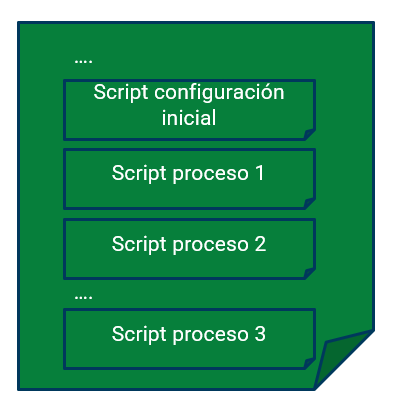
\includegraphics[width=5.46in]{images-1/02/scriptsecuenciador} \caption{Presentación esquematizada del funcionamiento de un script secuenciador}\label{fig:scriptsecuenciador}
\end{figure}

¿Cuántos scripts secuenciadores existen? El número total asciende a once porque actualmente hay un script secuenciador para la actualización de indicadores de la ENOE, otro para indicadores del IMSS, otro para indicadores del Censo Económico y otro tres para el módulo II, concretamente para consulta al DNE, SIAPI y el matching:

Módulo I

\begin{enumerate}
\def\labelenumi{\arabic{enumi})}
\item
  Script secuenciador para ENOE
\item
  Script secuenciador para IMSS
\item
  Script secuenciador para Censo
\end{enumerate}

Módulo II

\begin{enumerate}
\def\labelenumi{\arabic{enumi})}
\setcounter{enumi}{3}
\item
  Script secuenciador de consulta al DNE
\item
  Script secuenciador de matching coyuntural
\item
  Script secuenciador de predicción de riesgo
\end{enumerate}

Módulo IV

\begin{enumerate}
\def\labelenumi{\arabic{enumi})}
\setcounter{enumi}{6}
\item
  Script secuenciador para ENOE
\item
  Script secuenciador para IMSS\footnote{El lector percibirá que no hay un script secuenciador del censo económico histórico. Esto se debe a que dichos indicadores no entran al entrenamiento del modelo, como se describe en el módulo IV.}
\item
  Script secuenciador de consulta de histórico de inspecciones
\item
  Script secuenciador de matching histórico
\item
  Script secuenciador de entrenamiento de modelo
\end{enumerate}

En sentido estricto, un análisis más minucioso de los contenidos de este script permitiría sostener que algunos de los scripts arriba definidos como secuenciadores (en el sentido de que organizan el procesamiento de la información recurriendo a otros scripts para la consecución sus objetivos) realmente no tienen esta característica específica de ``llamar'' a otros scripts, sin embargo, a fines de presentación se simplifica su sistematización llamándolos como tal.

Así, uniendo los conceptos descritos en este y el anterior apartado, se puede presentar la ilustración \ref{fig:secConfigInicial} en la que se observa cómo un script secuenciador llama al script de configuración inicial, éste a su vez llama al \emph{0\_funciones\_catalogos} para luego a partir de un script de extracción se lamen los inputs para su transformación, y luego, cuando aplique, los scripts del cálculo de los indicadores, para dar con el output final.

\begin{figure}
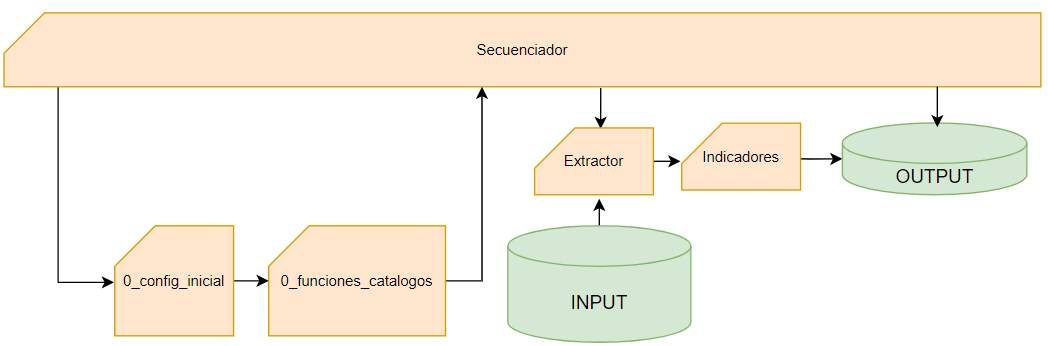
\includegraphics[width=14.56in]{images-1/02/sec_config_inicial} \caption{Presentación esquematizada de la relación }\label{fig:secConfigInicial}
\end{figure}

\hypertarget{estructuracarpetas}{%
\subsection{Estructura de carpetas y sintaxis de archivos}\label{estructuracarpetas}}

Dada la división de instrucciones en los diferentes scripts que fueron enunciados de manera genérica en la sección anterior, la estructura de las carpetas con que trabaja el SIDIL se describe en esta sección.

La organización de archivos en estas carpetas es agnóstica al sistema operativo y ubicación del SIDIL, siempre y cuando se transfiera el conjunto de carpetas sin realizar modificaciones. De realizarse cambios en los nombres de las carpetas, es muy probable que muchos scripts no funcionen, toda vez que los nombres de las carpetas son parte sustantiva de la identificación de inputs, scripts y outputs que se deben correr. De la misma manera, el cambio en el nombre de algunos archivos, particularmente los catálogos que no llevan una versión en el nombre del archivo, puede requerir ajustes en el código.\footnote{En estos casos, para mantener el control de versiones, al resguardar la versión anterior del catálogo, se le agrega la fecha de resguardo de dicha versión ``anterior'' al nombre del archivo. Ver Recuadro 8.}

En algunas carpetas específicas, particularmente las de la subcarpeta de insumos, la estructura ramificada incluye una subcarpeta final llamada ``anteriores'' que permite almacenar versiones anteriores de los objetos. Esto es particularmente útil para el procesamiento de catálogos toda vez que el código de lectura de catálogos busca específicamente un nombre determinado y todas las versiones anteriores a dicho catálogo deben estar almacenadas en la subcarpeta anteriores.

Cuarto, hay un script que genera esta estructura de carpetas a partir del catálogo de carpetas, el cual crea las carpetas, de no existir alguna de estas.

Hay cuatro grandes carpetas: 1\_insumos, 2\_codigos, 3\_resultados, 4\_reportes.

\begin{figure}
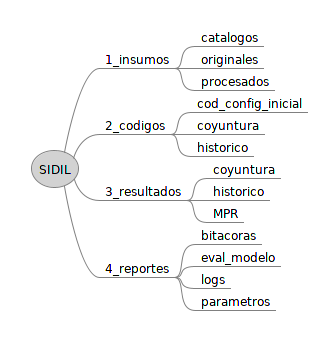
\includegraphics[width=4.62in]{images-1/03/organizacion_catalogos} \caption{Organización básica de las principales carpetas}\label{fig:organizacioncatalogos}
\end{figure}

Al interior de 1\_insumos se encuentran tres subcarpetas:

\begin{itemize}
\item
  La primera, \emph{catalogos}, reúne los diferentes archivos que sistematizan y etiquetan la información. Sobre ello se profundiza en la sección 3.9.
\item
  La segunda es \emph{originales} y sirve para depositar las fuentes de información sin procesamiento previo, por ejemplo, los archivos originales en formato dbf que componen la ENOE, o los archivos separados por tabulados que componen los registros administrativos del IMSS.
\item
  En la tercer subcarpeta, de nombre \emph{procesados}, se almacenan los resultados del procesamiento que ya forma parte del SIDIL, concretamente, el resultado de la extracción y transformación de cada fuente de información, siempre que se requiera el guardado de los temporales procesados.

  \begin{itemize}
  \tightlist
  \item
    Notar que en el caso de la ENOE, dado que su procesamiento no demanda mucha RAM, no se escribe a disco en esta carpeta. En contraste, para el procesamiento del IMSS se escriben tanto archivos temporales intermedios (que se borran luego de su utilización de manera automática) como también el guardado de los procesados ``finales'' (sin que estos sean resultados, sino que únicamente ``preprocesados'' que reducen las dimensiones y ``limpian'' algunos campos de los insumos).
  \end{itemize}
\end{itemize}

Al interior de \emph{2\_codigos}, existen tres principales subcarpetas:

\begin{itemize}
\item
  \emph{cod\_config\_inicial}: almacena el script \emph{0\_config\_inicial}, y el script \emph{0\_funciones\_catalogos} que se corren de manera anidada como parte de la ejecución de los scripts secuenciadores
\item
  \emph{coyuntura:} almacena en sus respectivas subcarpetas, los scripts que se requieren para la explotación de las diferentes fuentes de información. Por ejemplo, para la explotación de las fuentes de información ENOE e IMSS hay carpetas asignadas para almacenar, respectivamente, el script secuenciador, el script de extracción y transformación, los scripts de indicadores y los scripts de reportes.
\item
  \emph{historico:} lo mismo que \emph{coyuntura} pero a fines de la construcción histórica de los indicadores.
\end{itemize}

En la carpeta \emph{3\_resultados} se distinguen tres subcarpetas:

\begin{itemize}
\item
  \emph{coyuntura}: contiene subcarpetas para los cálculos de indicadores y las consultas al DNE
\item
  \emph{historico:} similar al caso anterior, pero con la consideración histórica
\item
  \emph{MPR:} El principal resultado del SIDIL, todas las versiones de ellas.
\end{itemize}

En la carpeta \emph{4\_reportes} se albergan cuatro subcarpetas

\begin{itemize}
\item
  \emph{bitacoras:} contiene dos archivos, ambos en formato tabular: Una bitácora donde se registran todas las ejecuciones de todos los scripts secuenciadores, y una bitácora de estatus donde se registra únicamente la última ejecución de cada script. El primero hace a la trazabilidad del sistema, mientras que el segundo permite mantener actualizada una tabla que se despliega en la interfaz de consulta y que informa, justamente, la última ejecución de cada proceso. Estos archivos, respectivamente, se llaman bitácora y bitácora\_estatus y están en formato csv.
\item
  \emph{eval\_modelo:} contiene los reportes de evaluación del modelo entrenado
\item
  \emph{Logs:} resguarda los logs (archivos .txt) que contienen los resultados y mensajes de la consola cuando se ejecutan los scripts
\item
  \emph{parametros: es la exportación de los parámetros que se definen en el script de configuración inicial.}
\end{itemize}

\hypertarget{temporalidad}{%
\subsection{Sobre la temporalidad}\label{temporalidad}}

A lo largo de la operación del SIDIL la persona usuaria podrá encontrar referencias a un periodo o momento exacto en el tiempo:

\begin{itemize}
\item
  Por un lado, está la referencia a la temporalidad que corresponde al periodo de representatividad de la medición o estimación de un fenómeno laboral. Por ejemplo, el primer trimestre de la ENOE, o el 31 de marzo de cierto año para los registros administrativos del IMSS.
\item
  Por otro lado, está la referencia a la versión de un elemento, sea un script, output o incluso input, que da cuenta de la fecha de su creación y/o última modificación. Por ejemplo, un script puede sufrir cambios y, para asegurar la trazabilidad de cada cálculo, debe guardarse con una versión distinta a la anterior.
\end{itemize}

El SIDIL, a lo largo de los diferentes módulos, está configurado para procesar o utilizar la última versión de un objeto, independientemente de su periodo de referencia. Es decir, toma la fecha de modificación que forma parte del nombre del archivo. Por eficiencia, lo más sensato es recurrir a la fecha de modificación.

En cambio, el formato de la referencia al periodo temporal es específico para cada fuente de información, toda vez que la frecuencia de actualización y representatividad es específica a cada fuente. Así por ejemplo la tabla con la información sociodemográfica de las personas encuestadas en la ENOE contiene en su nombre ``1t2022'' haciendo referencia al primer trimestre de 2022. En cambio, para el IMSS; cuya información original es de frecuencia mensual, la referencia es 2022131 (que representa la fecha de corte al 31 de enero de 2022).

Recuadro 6: Versionado de elementos

\begin{longtable}[]{@{}
  >{\raggedright\arraybackslash}p{(\columnwidth - 0\tabcolsep) * \real{1.0011}}@{}}
\caption{El versionado de los archivos no solo permite la trazabilidad (ver subsección siguiente) sino que además es indispensable para el funcionamiento adecuado del SIDIL. Dos ejemplos: primero, la lectura de scripts de cálculo de indicadores en el módulo I requiere la identificación de fecha (tan solo para poder aplicarlo, pero además para identificar la versión más reciente). De la misma manera, la interfaz de explotación de datos requiere del adecuado versionado de la MPR para poder identificar la versión más reciente y ofrecer la predicción de riesgos más actualizada.}\tabularnewline
\toprule\noalign{}
\begin{minipage}[b]{\linewidth}\raggedright
\textbf{El principio de versionado para todos los elementos en SIDIL es que la última versión de dicho elemento es la que se debe utilizar,} motivo por el cual, en el nombre del elemento (así como se guarda en las carpetas referidas) se debe incluir la fecha.

El formato de definición de la fecha que se utiliza para identificar la versión únicamente será el siguiente: \emph{aaaa\_mm\_dd\_hhmm}, es decir, cuatro dígitos para el año, seguido de un guion bajo, luego dos dígitos para el mes, otro guion bajo, luego dos dígitos para el día, otro guion bajo, y dos dígitos de la hora~ y dos de la hora juntos. Notar que la hora es en formato 24 horas. Por ejemplo: 2022\_11\_03\_0901 (año 2022, mes noviembre, día 03, 09 horas con 01 minutos). Este versionado se actualiza y genera automáticamente mediante el script de configuración inicial. La fecha y hora se obtiene directamente del sistema.

Para los scripts, el versionado también se incluye en el nombre del script al guardarlo; no es necesario incluir la hora y minuto del guardado pero sí mantener la estructura \emph{aaaa\_mm\_dd} de la fecha. Notar que el guardado de scripts se realiza de manera manual, toda vez que se consideran relativamente estables en el SIDIL y que justamente por eso el versionado de scripts no lleva horas ni minutos Es decir, cada cambio que se realice al script, se sugiere enfáticamente, debe culminar con el guardado de una nueva versión con una fecha posterior (al menos un día) a la versión anterior. El SIDIL está configurado para que scripts como el secuenciador, busquen la última versión de los diferentes scripts. En consecuencia:~ si hay dos elementos con el mismo nombre, se utiliza el que tenga la fecha de edición más reciente. Esta regla aplica para toda lectura de insumos.

Esto debe distinguirse del periodo de referencia, cuyo formato es específico a las fuentes de información utilizadas. Por ejemplo, en la ENOE se utiliza 1t2022, mientras que en el IMSS se utiliza 2022131 para enero de 2022.
\end{minipage} \\
\midrule\noalign{}
\endfirsthead
\toprule\noalign{}
\begin{minipage}[b]{\linewidth}\raggedright
\textbf{El principio de versionado para todos los elementos en SIDIL es que la última versión de dicho elemento es la que se debe utilizar,} motivo por el cual, en el nombre del elemento (así como se guarda en las carpetas referidas) se debe incluir la fecha.

El formato de definición de la fecha que se utiliza para identificar la versión únicamente será el siguiente: \emph{aaaa\_mm\_dd\_hhmm}, es decir, cuatro dígitos para el año, seguido de un guion bajo, luego dos dígitos para el mes, otro guion bajo, luego dos dígitos para el día, otro guion bajo, y dos dígitos de la hora~ y dos de la hora juntos. Notar que la hora es en formato 24 horas. Por ejemplo: 2022\_11\_03\_0901 (año 2022, mes noviembre, día 03, 09 horas con 01 minutos). Este versionado se actualiza y genera automáticamente mediante el script de configuración inicial. La fecha y hora se obtiene directamente del sistema.

Para los scripts, el versionado también se incluye en el nombre del script al guardarlo; no es necesario incluir la hora y minuto del guardado pero sí mantener la estructura \emph{aaaa\_mm\_dd} de la fecha. Notar que el guardado de scripts se realiza de manera manual, toda vez que se consideran relativamente estables en el SIDIL y que justamente por eso el versionado de scripts no lleva horas ni minutos Es decir, cada cambio que se realice al script, se sugiere enfáticamente, debe culminar con el guardado de una nueva versión con una fecha posterior (al menos un día) a la versión anterior. El SIDIL está configurado para que scripts como el secuenciador, busquen la última versión de los diferentes scripts. En consecuencia:~ si hay dos elementos con el mismo nombre, se utiliza el que tenga la fecha de edición más reciente. Esta regla aplica para toda lectura de insumos.

Esto debe distinguirse del periodo de referencia, cuyo formato es específico a las fuentes de información utilizadas. Por ejemplo, en la ENOE se utiliza 1t2022, mientras que en el IMSS se utiliza 2022131 para enero de 2022.
\end{minipage} \\
\midrule\noalign{}
\endhead
\bottomrule\noalign{}
\endlastfoot
 \\
\end{longtable}

\hypertarget{trazabilidad}{%
\subsection{Sobre trazabilidad: bitácora, log y parámetros}\label{trazabilidad}}

En el diseño del SIDIL se tomó en consideración la necesidad de asegurar la trazabilidad de la información generada. A tal fin se incorporaron los siguientes elementos al procesamiento de la información a través de los scripts.

\begin{itemize}
\item
  Bitácora: existe una única bitácora en el SIDIL en la cual se registran \emph{todas} las ejecuciones de los scripts secuenciadores, recuperando la siguiente información sobre el procesamiento de ciertos scripts{[}\^{}5{]}, al concluirse su ejecución de manera exitosa.

  \begin{itemize}
  \item
    La información que se registra en la bitácora es la siguiente:

    \begin{itemize}
    \item
      Fecha y hora de la ejecución
    \item
      Usuario responsable de la ejecución
    \item
      Nombre del script corrido
    \item
      Resultado obtenido: mensaje que se genera específicamente para cada script
    \item
      Liga al archivo de log (lo observado en la consola durante el procesamiento)
    \item
      Liga a los parámetros (aquellos definidos por configuración inicial o los que surgieron durante el procesamiento de un script).
    \end{itemize}
  \item
    Por otro lado, existe una segunda bitácora, llamada \emph{bitacora\_estatus} donde únicamente se registra la última ejecución de algunos procesos, los cuales se informan en la interfaz de automatización.
  \end{itemize}
\item
  Log de cada script: como se puntualiza en el anexo, la ejecución de un script, sea en R o Python, genera mensajes que se imprimen a la consola. Esto permite al usuario analizar el avance de la ejecución, detectar posibles inconsistencias, atender diferentes mensajes de errores, advertencias e información errores, etc.
\item
  Archivo de parámetros definidos: son los objetos generados que se utilizan en los diferentes scripts y que se generan desde el script de configuración inicial.
\item
  Reportes de la evaluación del modelo: Para los reportes asociados a la evaluación de los modelos, se generarán sólo cuando haya más de un modelo a evaluar, por lo que se exportan en formato tabular los resultados para las diferentes submaterias, según diferentes umbrales, dichos datos se exportan en formato .html, con la etiqueta del umbral usado. Estos reportes se encuentran en \emph{4\_reportes/eval\_modelo}
\end{itemize}

\hypertarget{mensajesGeneral}{%
\subsection{Mensajes al usuario}\label{mensajesGeneral}}

Esta sección adelanta algunos detalles que, independientemente de la ejecución a partir de una interfaz paraguas para la ejecución (semi)automatizada de los diferentes procesos (Ver sección xxx), ya pueden ser confirmados.

A lo largo de su ejecución, los diversos procedimientos reportan mensajes al usuario a través de la consola del software. Estos mensajes pueden ser clasificados en los siguientes grupos:

\hypertarget{mensajesError}{%
\subsubsection{Mensajes de error}\label{mensajesError}}

Estos mensajes surgen cuando la ejecución del código no es como se espera y el proceso probablemente falle en una(s) parte(s) o toda su ejecución. Casi con seguridad no se cumplió con el propósito del proceso y el mismo se interrumpió.

En algunos casos el mensaje de error puede reunir dos o tres elementos. Como se observa en el ejemplo a continuación, un primer elemento es el que está escrito en español. Esto es porque en este caso se pudo prever que este tipo de error pudiera surgir. El segundo elemento es el que empieza con ``Error in \ldots{}'' y esta es la información de error que genera el propio sistema. El tercer elemento es el que empieza con ``Warning message\ldots{}'', cuya aparición depende del tipo de error. Sobre esto último es importante notar que la aparición de un mensaje de ``warning'' por si sólo en muchas ocasiones no es un error y sólo es una advertencia del propio sistema. El SIDIL anticipa mucho de estos warning a partir de ``encapsular'' ciertas partes del código en un TryCatch.

\begin{quote}
\emph{``2022-12-22 13:19:13 ***ERROR***: No fue posible guardar el ultimo insumo de Accidentes (STPS\_RT\_202212.xlsx) debido a: Error in gzfile(file, mode): cannot open the connection}
\end{quote}

\emph{Warning message:}

\begin{quote}
\emph{In gzfile(file, mode) : cannot open compressed file `\ldots/SIDIL\_impaq/1\_insumos/procesados/coy\_IMSS\_acac/accidentes\_202212\_2022\_12\_22\_09\_37\_50.Rds', probable reason `No such file or directory'``}
\end{quote}

Notar que no siempre estarán los tres elementos en un mensaje de error. Podría ser un error no previsto, en cuyo caso no habrá un texto en español, o bien el propio sistema podría no arrojar el tercer elemento (``\emph{Warning\ldots{}}'') toda vez que no lo prevé así este lenguaje.

\hypertarget{mensajesAdvertencia}{%
\subsubsection{Mensajes de advertencia}\label{mensajesAdvertencia}}

Son mensajes que requieren la atención del usuario pero que no necesariamente implican que algo haya salido mal, y que no impiden que el procedimiento se desarrolle. Por ejemplo, en el procesamiento de los insumos más recientes de los registros administrativos del IMSS, se notifica al usuario si los periodos de referencia de los dos insumos que se deben ``cruzar'' (puestos asegurados y patrones registrados) no se refieren al mismo periodo de referencia. En dicho caso, el mensaje se despliega como:

\begin{quote}
\emph{``2022-12-22 12:45:15 ***ADVERTENCIA***: el periodo de referencia para insumos Patrones y Puestos no coincide.''}
\end{quote}

Como se explica más adelante, esto pudiera ser intencional o no y requiere la atención de una persona especialista para evaluar si es pertinente o se requieren ajustar, en este caso, los insumos puestos a disposición del SIDIL.

Notar que tanto los mensajes de error como de advertencia son acompañados, cuando previstos por el sistema, con tres asteriscos antes y después del tipo de error. Esto para propiciar su identificación en la consola.

\hypertarget{mensajesConfirmacion}{%
\subsubsection{Mensajes de información o de confirmación}\label{mensajesConfirmacion}}

Son mensajes que en la mayoría de las veces sólo informan al usuario el inicio o conclusión de algún proceso, mismo que anticipa qué estará procesando la computadora. Un ejemplo es:

\begin{quote}
\emph{2022-12-22 12:49:34 INFO: Se comienza lectura de insumo Accidentes: STPS\_RT\_202212.xlsx - periodo: 202212. El archivo pesa: 0.017 Mb}
\end{quote}

En este caso en particular, el peso del archivo puede ser indicativo del tiempo esperado para la ejecución completa de esta sección del código.

\hypertarget{software-para-el-procesamiento-de-datos}{%
\subsection{Software para el procesamiento de datos}\label{software-para-el-procesamiento-de-datos}}

El conjunto de scripts sobre los cuales descansa el SIDIL han sido desarrollados en R o Python, con el objetivo de aprovechar al máximo las ventajas que ofrecen ambos tipos de lenguaje de programación. La selección de estos lenguajes de programación obedece a la necesidad de escoger software libre, en línea con la Estrategia Digital Nacional (DOF 2021). Además, existen muchas razones por las que R y Python son populares en el área de la ciencia de datos, entre ellas, la disponibilidad de paquetes y librerías especializadas en la ciencia de datos que ahorran tiempo de programación a un usuario; una amplia comunidad de usuarios y una gran cantidad de recursos disponibles en línea, incluyendo libros, tutoriales y documentación; la posibilidad de integrar, a futuro, estos lenguajes con otras herramientas y plataformas como gestores de bases de datos, herramientas de visualización de datos, etc.

En el caso R, se utiliza la versión 2022.07.2+576 o superior (la última disponible a diciembre 2022 es 2022.12.0+353). Para más información ver Anexo 1. 8. En el caso de Python se utiliza la versión 3.10.8.

\hypertarget{catalogos}{%
\subsection{Catálogos de información}\label{catalogos}}

A lo largo del SIDIL se utilizan diversos catálogos de información que contienen información necesaria para la ejecución de los procesos. A excepción del catálogo de catálogos en particular, todos los catálogos se encuentran en su respectiva subcarpeta al interior de \emph{1\_insumos/catalogos}. El catálogo de catálogos (\emph{cat\_catalogos}) tiene como propósito caracterizar el contenido y ubicación de los diferentes catálogos, lo cual se aprovecha para la lectura de estos. Es un insumo clave para que la interfaz de automatización de la operación del SIDIL pueda resguardar adecuadamente potenciales nuevas versiones que reemplacen los catálogos anteriores.

El resto de los catálogos están organizados en subcarpetas según el tipo de información que contienen. Los nombres de las subcarpetas se indican en paréntesis.

\begin{enumerate}
\def\labelenumi{\arabic{enumi}.}
\item
  Relativos a la clasificación industrial (subcarpeta: \emph{clasificacion\_industrial}):

  \begin{enumerate}
  \def\labelenumii{\alph{enumii}.}
  \item
    Catálogo de correspondencia entre SCIAN Hogares y SCIAN México (subcarpeta \emph{SCIAN\_HOGARES}, archivo: \emph{cat\_scianHOGARES}): este catálogo establece la relación entre el catálogo de clasificación industrial SCIAN para hogares 2018, utilizado en la ENOE, y el catálogo SCIAN a nivel nacional 2018 a 3 dígitos. Si se llega a actualiza el catálogo SCIAN nacional es muy probable que se actualice también el catálogo SCIAN para hogares, por lo que se tendrá que realizar nuevamente esta homologación (conservando el mismo nombre del archivo).
  \item
    Catálogo de correspondencia entre IMSS y SCIAN México (subcarpeta \emph{IMSS\_SCIAN}, archivo: \emph{cat\_correspondencia\_IMSS4\_SCIAN2ySCIAN3\_2018}): Este catálogo establece una relación unidireccional entre la clasificación de actividades siguiendo la taxonomía del IMSS y la del SCIAN 2018 a nivel nacional, a dos y tres dígitos. Es decir, dado el campo de clasificación de actividades que ofrecen los registros administrativos del IMSS, a través de este catálogo se reclasifica dicha actividad para expresarla en la taxonomía del SCIAN. Este catálogo resume los diferentes esfuerzos de comparativa de taxonomías realizados tanto en la STPS como en AIR.
  \item
    Catálogo de clasificación de actividades industriales siguiendo el sistema del IMSS (subcarpeta \emph{IMSS}, archivo: \emph{cat\_actividades\_IMSS}): Este catálogo es, en esencia, la información contenida en el diccionario de datos del IMSS llamado ``Diccionario de datos puestos de trabajo afiliados y asegurados sin un empleo asociado / Diccionario de datos asegurados'' disponible en IMSS (2023)
  \item
    Catálogo de clasificación de actividades siguiendo el SCIAN 2018 (subcarpeta \emph{SCIAN}, archivo: \emph{cat\_activ\_SCIAN}), conforme publicado por INEGI (2018a). Consultar también las tablas comparativas en INEGI (2018b)
  \end{enumerate}
\item
  Relativos a campos en las fuentes de información (\emph{fuentes\_informacion})

  \begin{enumerate}
  \def\labelenumii{\alph{enumii}.}
  \item
    Catálogo de campos (subcarpeta \emph{nombres\_campos}, archivo: \emph{cat\_nombre\_campos}): es una tabla para ENOE e IMSS que permite asociar de manera unívoca diferentes nombres del mismo concepto, para, por ejemplo, atender a cambios que ocurrieron en las bases originales a lo largo del tiempo. Por poner un caso: en algunas bases más antiguas (aproximadamente año 2019) el IMSS llamaba como ``cve\_patron'' al campo ``registro patronal'', nombre que sostiene desde el año 2020. El catálogo permite unificar todas las diferentes versiones de nombre del mismo campo a uno solo. Así, de presentarse nuevos cambios a los campos, sólo es necesario actualizar este catálogo y no todos los códigos. Imagine modificar más de 30 veces el nombre del campo ``registro'' y asegurar su consistencia a lo largo del tiempo. En este catálogo, el campo \emph{nombre\_anterior} refiere al nombre que originalmente es proporcionado por la fuente de información en la versión original de los datos. El campo \emph{nombre\_nuevo} registra el nombre con el que se procesará la información a lo largo del código.
  \item
    Catálogo de fuentes de información (subcarpeta \emph{fuentes}, archivo: \emph{cat\_fuentes}). Este catálogo estipula parámetros que se requieren para que la interfaz de automatización resguarde adecuadamente los insumos de datos, a su vez que se debe mantener actualizado para que, a partir de este archivo, se permita la incorporación de nuevas fuentes de información.
  \end{enumerate}
\item
  Relativos a información generada durante el procesamiento de información (\emph{procesamiento\_informacion})

  \begin{enumerate}
  \def\labelenumii{\alph{enumii}.}
  \item
    El catálogo de organización de carpetas (subcarpeta \emph{organización\_carpetas}, archivo \emph{cat\_organizacion\_carpetas}). Este catálogo contiene toda la estructura de carpetas del SIDIL, el cual es consultado para verificar la existencia de las carpetas o, si es el caso, crearlas. Este es el único catálogo que no se encuentra en la carpeta de insumos, sino que se alberga junto con el proyecto R.
  \item
    Catálogo de indicadores (subcarpeta \emph{indicadores,} archivo \emph{cat\_indicadores}). Este catálogo contiene los indicadores calculados que se utilizan en el SIDIL para el entrenamiento y la predicción del riesgo de los CT. Consta de las siguientes columnas: \emph{fuente}, \emph{indicador} (nombre que le fue asignado), \emph{etiqueta} (breve descripción del indicador), \emph{entra\_al\_modelo} (con opciones de si y no que indica aquellos indicadores que toma en cuenta el modelo predictivo), \emph{especificación} (a qué tipo de combinación de tablas aplica en la fuente de información original, específicamente para indicadores del IMSS). \emph{umbral\_cv} representa el máximo nivel del coeficiente de variación que se acepta en una estimación puntual, particularmente importante para la explotación de muestras complejas. \emph{referencia} es el nivel de significancia para la detección de outliers al comparar estimaciones puntuales coyunturales contra valores de referencia construiídos a partir de \emph{etiqueta\_MPR} y \emph{descripcion\_MPR} son para la caracterización en la MPR. Notar que cualquier cambio en los indicadores (supresión o incorporación de nuevos indicadores o cambios en alguno de los campos) debe ser reflejado en este archivo.
  \item
    Catálogo de niveles de agregación (subcarpeta \emph{niveles\_agregacion}, archivo \emph{cat\_niveles\_agregacion}): especifica los diferentes niveles de agregación según la especificidad de los campos de clasificación industrial (a dos y tres dígitos, \emph{scian2018\_2} y \emph{scian2018\_3}, respectivamente), de geografía (geo2- a nivel estatal- y geo5 - municipal) y de categoría de tamaño (\emph{cat\_tamanio}).
  \item
    Catálogo de categorías de tamaño (subcarpeta \emph{tamanio}, archivo: \emph{cat\_tamanio)}: el catálogo contiene las seis categorías de tamaño de los CT estipulados en el SIDIL. La tabla cuenta con cinco columnas: \emph{cat\_tamanio} (enumeración del 1 al 6), \emph{etiq\_cat\_tamanio} (la etiqueta del rango de tamaño para cada enumeración), \emph{estrato\_censo\_economico} (la homologación entre el campo \emph{estrato} del Censo Económico y el campo \emph{cat\_tamanio}), \emph{p3q\_en\_enoe} (la homologación entre el campo \emph{p3q} de la ENOE y el campo \emph{cat\_tamanio}) y \emph{corte\_numerico} (la homologación entre los datos del IMSS y el campo \emph{cat\_tamanio}). Si llegase a cambiar alguna de las categorías de alguna de las fuentes, los cambios correspondientes se deben hacer directamente en este catálogo.
  \item
    Catálogo de campos del DNE (subcarpeta \emph{campor\_DNE}, archivo: \emph{cat\_campos\_DNE).} El catálogo contiene los campos que serán recuperados del DNE a lo largo de los diferentes scripts. Cuenta con cinco columnas: \emph{fuente} (DNE en todos los casos), \emph{indicador} (con el nombre del campo), \emph{etiqueta} y \emph{entra\_al\_modelo} (con opciones de si y no para entrar al modelo predictivo), \emph{tabla} (la entidad dentro de la base de datos relacional). Con el campo \emph{tipo} se escpecifica que tipo de filtro aplica al explotar estos campos (que luego en la MPR son atributos de los CT del DNE) a través de la interfaz de consulta.
  \item
    Catálogo de campos del SIAPI SIPAS (subcarpeta \emph{campos\_SIAPISIPAS}, archivo: \emph{cat\_campos\_SIAPISIPAS}): Contiene los campos y ubicación de los mismos dentro del sistema SIAPI SIPAS.
  \item
    Catálogo de procesos (directamente en la subcarpeta \emph{procesamiento\_informacion}): Este catálogo identifica los procesos que se pueden ejecutar desde la interfaz de automatización.
  \end{enumerate}
\item
  Relativos al marco geoestadístico (subcarpeta \emph{marco\_geoestadistico)}:

  \begin{enumerate}
  \def\labelenumii{\alph{enumii}.}
  \item
    Catálogo de entidades y municipios IMSS e INEGI (subcarpeta \emph{municipiosIMSS\_INEGI,} archivo\emph{: municipios\_imss\_inegi}). El IMSS utiliza una clasificación de municipios distinta al marco geoestadístico del INEGI, motivo por el cual este catálogo establece la relación unidireccional de municipios siguiendo la taxonomía del IMSS a municipios siguiendo la taxonomía del INEGI.
  \item
    Catálogo de entidades y municipios DNE e INEGI (subcarpeta \emph{municipios\_dne\_inegi,} archivo\emph{: cat\_municipiosDNE\_INEGI}). El DNE utiliza una clasificación de municipios distinta al marco geoestadístico del INEGI, motivo por el cual este catálogo establece la relación unidireccional de municipios hacia la taxonomía del INEG.
  \item
    Municipios frontera norte (subcarpeta: \emph{municipios\_fn}, archivo: \emph{cat\_municipiosFronteraNorte}): los centros de trabajo operando en municipios en la Zona Libre de la Frontera Norte tienen estipulado un salario mínimo distinto al del resto del país. Este catálogo expresa con una variable indicativa dicha pertenencia. La información original viene de este \href{https://www.gob.mx/se/acciones-y-programas/zona-libre-de-la-frontera-norte}{enlace}.
  \item
    Áreas urbanas (subcarpeta \emph{áreas\_urbanas}, archivo: \emph{areasurbanas}): este catálogo identifica los municipios que, según el INEGI, forman parte de un área urbana. Es, fundamentalmente, utilizado para el cálculo de concentración de mercado.
  \item
    Correspondencia de municipios entre el DNE y el INEGI (subcarpeta \emph{municipios\_dne\_inegi}, archivo \emph{cat\_municipiosDNE\_INEGI}): Esto atiende a la realidad de que en el DNE no se utilizó el marco geoestadístico oficial. Por lo que este catálogo permite transitar de la clave de municipio registrada en DNE al marco geoestadístico oficial en México. Actualmente se encuentra asociado al marco geoestadístico de INEGI versión 2023/01, disponible en INEGI (2023).
  \end{enumerate}
\item
  Relativo al marco normativo

  \begin{enumerate}
  \def\labelenumii{\alph{enumii}.}
  \tightlist
  \item
    Catálogo de materias y submaterias que forman parte del potencial alcance de una inspección (subcarpeta \emph{marco\_normativo}, archivo: \emph{cat\_submaterias)}. Establece la relación entre el código identificador de submaterias y materias de inspección con las etiquetas.
  \end{enumerate}
\end{enumerate}

Recuadro 8: Versiones de archivos de catálogos.

\begin{longtable}[]{@{}
  >{\raggedright\arraybackslash}p{(\columnwidth - 0\tabcolsep) * \real{1.0028}}@{}}
\caption{La Matriz de Predicción de Riesgo}\tabularnewline
\toprule\noalign{}
\begin{minipage}[b]{\linewidth}\raggedright
Si se requiere hacer algún cambio sobre la información que abarca los catálogos este se debe hacer directamente en los mismos catálogos, pero se sugiere sea de la siguiente manera:

\begin{enumerate}
\def\labelenumi{\arabic{enumi})}
\item
  Resguardar una copia del catálogo desactualizado en la subcarpeta \emph{anteriores\_descartar} que se encuentra en su respectiva carpeta. Se sugiere guardarlo con la fecha en la que dicho catalogo fue reemplazado.
\item
  Modificar y/o reemplazar el catálogo, para que esta sea procesada correctamente por los scripts, sin cambiar el nombre del archivo del catálogo.
\end{enumerate}

Por ejemplo, si se desarrolla un nuevo indicador que quiere ser integrado al SIDIL, no solo se deben desarrollar sus códigos y guardarlos en las carpetas correspondientes, también debe ser agregado al catálogo de indicadores (\emph{cat\_indicadores}), o si cambia el marco normativo, este se debe actualizar en su respectiva carpeta de catálogos (\emph{marco\_normativo}).

De ser necesario, es posible resguardar la versión anterior del catálogo, entonces puede resguardarse en la subcarpeta \emph{anteriores}. Lo importante es que el script de configuración inicial, siempre "buscará" el mismo nombre de archivo insumo para cada catálogo, independientemente de su contenido o vigencia.

Precisando esto último, la carga de los diferentes catálogos será a partir de la información resguardada en el catálogo de catálogos, mismo que se encuentra en la raíz del proyecto. Esto es importante porque la consistencia de nombres que se estipula a lo largo del SIDIL también requiere tomar este archivo en consideración.
\end{minipage} \\
\midrule\noalign{}
\endfirsthead
\toprule\noalign{}
\begin{minipage}[b]{\linewidth}\raggedright
Si se requiere hacer algún cambio sobre la información que abarca los catálogos este se debe hacer directamente en los mismos catálogos, pero se sugiere sea de la siguiente manera:

\begin{enumerate}
\def\labelenumi{\arabic{enumi})}
\item
  Resguardar una copia del catálogo desactualizado en la subcarpeta \emph{anteriores\_descartar} que se encuentra en su respectiva carpeta. Se sugiere guardarlo con la fecha en la que dicho catalogo fue reemplazado.
\item
  Modificar y/o reemplazar el catálogo, para que esta sea procesada correctamente por los scripts, sin cambiar el nombre del archivo del catálogo.
\end{enumerate}

Por ejemplo, si se desarrolla un nuevo indicador que quiere ser integrado al SIDIL, no solo se deben desarrollar sus códigos y guardarlos en las carpetas correspondientes, también debe ser agregado al catálogo de indicadores (\emph{cat\_indicadores}), o si cambia el marco normativo, este se debe actualizar en su respectiva carpeta de catálogos (\emph{marco\_normativo}).

De ser necesario, es posible resguardar la versión anterior del catálogo, entonces puede resguardarse en la subcarpeta \emph{anteriores}. Lo importante es que el script de configuración inicial, siempre "buscará" el mismo nombre de archivo insumo para cada catálogo, independientemente de su contenido o vigencia.

Precisando esto último, la carga de los diferentes catálogos será a partir de la información resguardada en el catálogo de catálogos, mismo que se encuentra en la raíz del proyecto. Esto es importante porque la consistencia de nombres que se estipula a lo largo del SIDIL también requiere tomar este archivo en consideración.
\end{minipage} \\
\midrule\noalign{}
\endhead
\bottomrule\noalign{}
\endlastfoot
 \\
\end{longtable}

La Matriz de Predicción de Riesgo (MPR) es un producto crítico del sistema. La MPR es la tabla que reúne el universo actualizado de centros de trabajo disponibles en el DNE (una fila de la matriz por cada centro de trabajo), junto con sus atributos más importantes, los indicadores atribuidos a ellos a partir de la explotación de diferentes fuentes de información, y por supuesto, la predicción de riesgo asociada a ciertas submaterias y una predicción de riesgo general (todo ello en las columnas de la matriz). Es, en esencia, el principal producto del SIDIL previo a la priorización de un subconjunto del universo de CT realizada por quien esté a cargo de la programación de inspecciones.

La MPR es un punto crítico porque:

\begin{enumerate}
\def\labelenumi{\arabic{enumi})}
\item
  Es el producto con el cual culmina el proceso a cargo de la DGIET, es decir, en donde concluye el procesamiento de información.
\item
  Contiene el resumen de toda la información extraída, generada o procesada a lo largo del ciclo del SIDIL para los centros de trabajo.
\item
  Junto con los metadatos asociados a la MPR, es el único insumo imprescindible para el funcionamiento de la interfaz de consulta.
\item
  Contiene toda la información que, a través de filtros y consultas, permitirá generar los universos susceptibles de ser inspeccionados, priorizados por riesgo de incumplimiento en las diferentes submaterias.
\end{enumerate}

\hypertarget{presentaciuxf3n-sintuxe9tica-de-todos-los-scripts}{%
\section{Presentación sintética de todos los scripts}\label{presentaciuxf3n-sintuxe9tica-de-todos-los-scripts}}

A continuación se presentan de manera sintética todos los scripts que constituyen el SIDIL.

\begin{longtable}[]{@{}
  >{\raggedright\arraybackslash}p{(\columnwidth - 12\tabcolsep) * \real{0.0551}}
  >{\raggedright\arraybackslash}p{(\columnwidth - 12\tabcolsep) * \real{0.0188}}
  >{\raggedright\arraybackslash}p{(\columnwidth - 12\tabcolsep) * \real{0.2522}}
  >{\raggedright\arraybackslash}p{(\columnwidth - 12\tabcolsep) * \real{0.2174}}
  >{\raggedright\arraybackslash}p{(\columnwidth - 12\tabcolsep) * \real{0.0217}}
  >{\raggedright\arraybackslash}p{(\columnwidth - 12\tabcolsep) * \real{0.1884}}
  >{\raggedright\arraybackslash}p{(\columnwidth - 12\tabcolsep) * \real{0.2391}}@{}}
\toprule\noalign{}
\begin{minipage}[b]{\linewidth}\raggedright
\textbf{Nombre (sin incluir versionado)}
\end{minipage} & \begin{minipage}[b]{\linewidth}\raggedright
\textbf{Módulo}
\end{minipage} & \begin{minipage}[b]{\linewidth}\raggedright
\textbf{Objetivo}
\end{minipage} & \begin{minipage}[b]{\linewidth}\raggedright
\textbf{Observaciones}
\end{minipage} & \begin{minipage}[b]{\linewidth}\raggedright
\textbf{Lenguaje}
\end{minipage} & \begin{minipage}[b]{\linewidth}\raggedright
\textbf{Principales insumos}
\end{minipage} & \begin{minipage}[b]{\linewidth}\raggedright
\textbf{Principales outputs}
\end{minipage} \\
\midrule\noalign{}
\endhead
\bottomrule\noalign{}
\endlastfoot
0\_config\_inicial & I a IV & \begin{minipage}[t]{\linewidth}\raggedright
Carga de paqueterías para ambiente R;\\
Define parámetros de explotación de información\strut
\end{minipage} & Es ejecutado por prácticamente todos los scripts secuenciadores & R & NA & Parámetros cargados en la memoria RAM \\
0\_funciones\_catalogos & I a IV & Define funciones & A excepción del script 9\_envio\_MPR, este script siempre es llamado por 0\_config\_inicial & R & Catálogos de información & Catálogos cargados y funciones definidas en la RAM. \\
1\_secuenciador\_ENOE & I & Ejecuta toda la rutina para generar los indicadores coyunturales de la ENOE & Es el único script que se debe ejecutar, ya que este llama a los otros scripts & R & Script de configuración inicial; catálogos; script de extracción; scripts de generación de indicadores & Una tabla por cada indicador calculado con las estimaciones puntuales de dicho indicador. Una tabla con los valores de referencia de cada indicador. \\
1\_extraccion\_ENOE & I & Construye la base de insumo para el cálculo de los indicadores de la ENOE a partir de las bases originales en formato .dbf & Se ejecuta automáticamente desde el script secuenciador & R & Tablas originales de la ENOE en formato .dbf & Una tabla unificada de la ENOE en formato .dbf con la población subordinada y reumunerada \\
1\_brecha\_gen\_ENOE & I & Genera las estimaciones puntuales coyunturales del indicador ``brecha de género'' de la ENOE & Se ejecuta automáticamente desde el script secuenciador & R & La tabla resultado del script de extracción & Una tabla con las estimaciones puntuales del respectivo indicador. \\
1\_contrato\_escrito\_ENOE & I & Genera las estimaciones puntuales coyunturales del indicador ``contrato escrito'' de la ENOE & Se ejecuta automáticamente desde el script secuenciador & R & La tabla resultado del script de extracción & \\
1\_dias\_trab\_ENOE & I & Genera las estimaciones puntuales coyunturales del indicador ``días trabajados'' de la ENOE & Se ejecuta automáticamente desde el script secuenciador & R & La tabla resultado del script de extracción & \\
1\_hrs\_trab\_ENOE & I & Genera las estimaciones puntuales coyunturales del indicador horas trabajadas'' de la ENOE & Se ejecuta automáticamente desde el script secuenciador & R & La tabla resultado del script de extracción & \\
1\_ing\_min\_ENOE & I & Genera las estimaciones puntuales coyunturales del indicador ``ingreso mínimo'' de la ENOE & Se ejecuta automáticamente desde el script secuenciador & R & La tabla resultado del script de extracción & \\
1\_ing\_x\_hrs\_ENOE & I & Genera las estimaciones puntuales coyunturales del indicador ``ingreso por hraso'' de la ENOE & Se ejecuta automáticamente desde el script secuenciador & R & La tabla resultado del script de extracción & \\
1\_ing\_x\_mes\_ENOE & I & Genera las estimaciones puntuales coyunturales del indicador ``ingreso por mes'' de la ENOE & Se ejecuta automáticamente desde el script secuenciador & R & La tabla resultado del script de extracción & \\
1\_presta\_soc\_ENOE & I & Genera las estimaciones puntuales coyunturales del indicador ``prestaciones sociales'' de la ENOE & Se ejecuta automáticamente desde el script secuenciador & R & La tabla resultado del script de extracción & \\
1\_seg\_soc\_ENOE & I & Genera las estimaciones puntuales coyunturales del indicador ``seguridad social'' de la ENOE & Se ejecuta automáticamente desde el script secuenciador & R & La tabla resultado del script de extracción & \\
1\_sindicato\_ENOE & I & Genera las estimaciones puntuales coyunturales del indicador ``sindicato'' de la ENOE & Se ejecuta automáticamente desde el script secuenciador & R & La tabla resultado del script de extracción & \\
1\_tipo\_contrato\_ENOE & I & Genera las estimaciones puntuales coyunturales del indicador ``tipo contrato'' de la ENOE & Se ejecuta automáticamente desde el script secuenciador & R & La tabla resultado del script de extracción & Una tabla con las estimaciones puntuales del indicador. \\
1\_secuenciador\_CENSO2019 & I & Ejecuta toda la rutina para generar los indicadores del Censo Económico & Es el único script del Censo Económico & R & Tabla de datos de las 3 empresas más grandes a nivel municipal y rama (SCIAN 2 dígitos), producto de la colaboración INEGI-STPS & Una tabla por cada indicador calculado con las estimaciones puntuales de dicho indicador. \\
1\_secuenciador\_IMSS & I & Ejecuta toda la rutina para generar los indicadores del IMSS & Es el único script que se debe ejecutar, ya que este llama a los otros scripts & R & Script de configuración inicial; catálogos; script de extracción; scripts de generación de indicadores & Una tabla por cada indicador calculado con las estimaciones puntuales de dicho indicador. Una tabla con los valores de referencia de cada indicador. \\
1\_extraccion\_IMSS & I & Construye la base de insumo para el cálculo de los indicadores del IMSS & Se ejecuta automáticamente desde el script secuenciador & R & Insumos originales del IMSS: accidenes (riesgos), patrones y puestos (asegurados) & Una tabla para cada insumo original por mes, además para puestos, una tabla adicional con los NSS de las personas aseguradas, también por mes. \\
1\_brecha\_imss & I & Genera las estimaciones puntuales coyunturales del indicador ``brecha salarial de género'' del IMSS & Se ejecuta automáticamente desde el script secuenciador & R & Insumos procesados, combinados selectivamente desde el secuenciador. & Estimaciones puntuales en dos tablas: por nivel de agregación y nominativo, para cada mes. \\
1\_concen\_mercado\_imss & I & Genera las estimaciones puntuales coyunturales del indicador ``concentración de mercado'' del IMSS & Se ejecuta automáticamente desde el script secuenciador & R & Insumos procesados, combinados selectivamente desde el secuenciador. & \\
1\_rot\_lab & I & Genera las estimaciones puntuales coyunturales del indicador ``rotación laboral'' del IMSS & Se ejecuta automáticamente desde el script secuenciador & R & Insumos procesados, combinados selectivamente desde el secuenciador. & \\
1\_salario\_minimo & I & Genera las estimaciones puntuales coyunturales del indicador ``rotación laboral'' del IMSS & Se ejecuta automáticamente desde el script secuenciador & R & Insumos procesados, combinados selectivamente desde el secuenciador. & \\
1\_tasa\_acc & I & Genera las estimaciones puntuales coyunturales del indicador ``rotación laboral'' del IMSS & Se ejecuta automáticamente desde el script secuenciador & R & Insumos procesados, combinados selectivamente desde el secuenciador. & \\
1\_tasa\_dias & I & Genera las estimaciones puntuales coyunturales del indicador ``rotación laboral'' del IMSS & Se ejecuta automáticamente desde el script secuenciador & R & Insumos procesados, combinados selectivamente desde el secuenciador. & \\
2\_consulta\_DNE\_ & II & Organiza la consulta al DNE (como secuenciador) y enriquece la categoría de tamaño con base en los patrones registrados ante el IMSS. & & R & DNE y Patrones del IMSS & DNE\_plus: universo de CT consultado del DNE. \\
2\_conexion & II & Establece la conexión al SQL Server. & Se ejecuta automáticamente desde 2\_consulta\_DNE & R & Credenciales de acceso a SQL Server & Conexión a DNE en la RAM \\
2\_extraccion\_DNE & II & Formula y envía queries para extraer tablas del SQL Server & Se ejecuta automáticamente desde 2\_consulta\_DNE & R & Catálogo de campos del DNE & Tablas consultadas al DNE, en la RAM \\
2\_matching\_coyuntural\_ & II & Imputa de manera nominativa y por nivel de agregación los indicadores coyunturales al DNE\_plus & & Python & DNE\_plus & Universo CT con indicadores coyunturales imputados \\
2\_prediccion\_modelo\_ & II & Genera predicción de riesgos por submateria y general & & Python & Universo CT con indicadores coyunturales imputados & Matriz de predicción de riesgos \\
automatizacion/app.R & I y II & Es la app de la interfaz de automatización que organiza la actualización de fuentes de información, carga de catálogos y la ejecución de los scripts en los módulos I y II. & La interfaz únicamente permite la realización de procesos del módulo I y II. & R & Todos los scripts y fuentes de información de los módulos I y II & Todos los outputs de los módulos I y II \\
consulta/app.R & III & Es la app de la interfaz de consulta que permite priorizar los CT con base en sus predicciones de riesgo, atributos e indicadores & & R & Matriz de predicción de riesgos & Universo de CT que satisfacen criterios de inspección \\
4\_query\_violaciones\_inspecciones\_ & IV & Organiza la consulta al SIAPI-SIPAS & Incluye la consulta al universo de CT para recuperar atributos de los mismos & R & Credenciales de acceso a SQL Server & Historico de inspecciones por submateria incluyendo si se encontraron violaciones que proceden \\
4\_secuenciador\_ENOE & IV & Ejecuta toda la rutina para generar los indicadores coyunturales de la ENOE & Es el único script que se debe ejecutar, ya que este llama a los otros scripts & R & Script de configuración inicial; catálogos; script de extracción; scripts de generación de indicadores & enoe\_historico\_v.Rds: una sola tabla con todos los indicadores para todos los años. \\
4\_extraccion\_ENOE & IV & Construye la base de insumo para el cálculo de los indicadores de la ENOE a partir de las bases originales en formato .dbf & La unica diferencia respecto a este script del módulo I es que en el módulo IV se incluye el año. & R & Tablas originales de la ENOE en formato .dbf & Una tabla unificada de la ENOE en formato .dbf con la población subordinada y reumunerada, con el año \\
4\_brecha\_gen\_ENOE & IV & Genera las estimaciones puntuales coyunturales del indicador ``brecha de género'' de la ENOE & & R & La tabla resultado del script de extracción. & El cálculo por año para cada indicador, mismo que luego el secuenciador ``apila'' para conformar una sola tabla con todos los indicadores. \\
4\_contrato\_escrito\_ENOE & IV & Genera las estimaciones puntuales coyunturales del indicador ``contrato escrito'' de la ENOE & & R & & \\
4\_dias\_trab\_ENOE & IV & Genera las estimaciones puntuales coyunturales del indicador ``días trabajados'' de la ENOE & & R & & \\
4\_hrs\_trab\_ENOE & IV & Genera las estimaciones puntuales coyunturales del indicador horas trabajadas'' de la ENOE & & R & & \\
4\_ing\_x\_hrs\_ENOE & IV & Genera las estimaciones puntuales coyunturales del indicador ``ingreso por hraso'' de la ENOE & & R & & \\
4\_ing\_x\_mes\_ENOE & IV & Genera las estimaciones puntuales coyunturales del indicador ``ingreso por mes'' de la ENOE & & R & & \\
4\_presta\_soc\_ENOE & IV & Genera las estimaciones puntuales coyunturales del indicador ``prestaciones sociales'' de la ENOE & & R & & \\
4\_seg\_soc\_ENOE & IV & Genera las estimaciones puntuales coyunturales del indicador ``seguridad social'' de la ENOE & & R & & \\
4\_sindicato\_ENOE & IV & Genera las estimaciones puntuales coyunturales del indicador ``sindicato'' de la ENOE & & R & & \\
4\_tipo\_contrato\_ENOE & IV & Genera las estimaciones puntuales coyunturales del indicador ``tipo contrato'' de la ENOE & & R & & \\
1\_secuenciador\_IMSS & IV & Ejecuta toda la rutina para generar los indicadores del IMSS & La unica diferencia respecto a este script del módulo I es en la configuración de parámetros & R & Script de configuración inicial; catálogos; script de extracción; scripts de generación de indicadores & Una tabla por cada indicador calculado con las estimaciones puntuales de dicho indicador. Una tabla con los valores de referencia de cada indicador. \\
4\_matching\_historico & IV & Imputa de manera nominativa y por nivel de agregación los indicadores históricos de IMSS y ENOE al histórico de inspecciones & & Python & Tablas de indicadores históricos del IMSS y de la ENOE; histórico de inspecciones por submateria que incluye atributos del DNE & UniversoInspeccionesInd\_v.Rds: una tabla que a cada inspección y submateria le asocia los valores históricos del IMSS y ENOE, además de los atributos del DNE. \\
4\_entrenamiento\_modelo & IV & Entrena el modelo random forest con base en el histórico de inspecciones. & Se pueden entrenar dos modelos, actualmente predefinido para que sea Random Forest. La alternativa es el Tabnet (red neuronal para datos tabulares) & Python & UniversoInspeccionesInd\_v.Rds & Modelo entrenado, exportado a archivos pkl, un txt con las variables de entrada del modelo, score y submateria con la métrica de ajuste de las predicciones (MAE). \\
4\_eval\_modelo & IV & Genera métricas de performance del modelo y análisis Shapley (medición de contribución relativa de variables de entrada). & & Python. & El modelo entrenado y la base histórica de inspecciones por submateria. & \begin{minipage}[t]{\linewidth}\raggedright
Dos tablas reportadas en el log con las métricas de performance.\\
Imágenes (png) con el análisis Shapley, mismas que además conforman un html.\strut
\end{minipage} \\
\end{longtable}

\hypertarget{r-rstudio-y-python}{%
\section{R, RStudio y Python}\label{r-rstudio-y-python}}

En este anexo se presentan, fundamentalmente, los conceptos y prácticas básicas en la utilización de la interfaz de RStudio. También se presentan algunos aspectos relevantes de Python, pero que si bien requiere tenerse instalado, desde la perspectiva de SIDIL, no requiere ser ejecutado en una interfaz distinta a Rstudio

\hypertarget{r-y-rstudio}{%
\subsection{R y RStudio}\label{r-y-rstudio}}

La gran mayoría de los algoritmos que constituyen el SIDIL se desarrollaron y mantendrán en el lenguaje R.\footnote{\url{https://www.r-project.org/about.html}} Esto es independiente de que a través de una interfaz ``paraguas'' se pudieran automatizar hasta cierto punto la secuencia de los scripts. R es el lenguaje de programación de uso libre desarrollado para el análisis estadístico y gráfico. Afortunadamente existe un ambiente integrado de desarrollo que se llama RStudio (que recientemente cambió su nombre a Posit\footnote{\url{https://posit.co/}}) y que facilita la programación, compilación y visualización de desarrollos en el lenguaje R. SIDIL prevé que el usuario procese la información con R Studio, y para que este último funcione se requiere tener R instalado. A continuación, se ofrecen detalles sobre las principales características de R y RStudio.

\hypertarget{el-entorno-de-rstudio}{%
\subsection{El entorno de RStudio}\label{el-entorno-de-rstudio}}

El entorno de RStudio está conformado por cuatro partes (ver ilustración \ref{fig:entornoRStudio}):

\begin{enumerate}
\def\labelenumi{\arabic{enumi}.}
\item
  Scripts: En esta parte se generan o cargan los scripts o archivos de código que se van a ejecutar. Se pueden abrir varios scripts a la vez. Todos los scripts, independientemente de que estén en pestañas separadas, utilizan y cargan objetos del mismo ambiente (a menos que se configure distinto, cosa que no sucede en SIDIL). Para correr una línea de un script se debe poner el cursor sobre la línea que se desee correr y presionar la tecla Control (Ctrl) + Intro o se puede presionar el botón ``Run'' en la parte izquierda superior de esta sección. Para ejecutar el script completo se debe presionar Ctrl + Shift + Intro. Se pueden seleccionar con el cursor las líneas que se deseen correr y presionar Ctrl+Intro o la tecla Run. Para aquellas/os lectores más familiarizados con Stata, el equivalente a un script en dicho software es el ``do file''.
\item
  Ambiente (Environment): En el ambiente se muestran todos los objetos generados por los códigos. Es importante mencionar que los objetos que se alojan en el ambiente no están guardados en el disco rígido del equipo de cómputo, únicamente están disponibles en esta sección mientras se ejecutan los scripts. Para el guardado de los elementos se debe generar el comando correspondiente en el script o consola, determinando el cómo se quiere guardar el objeto generado. Para eliminar un objeto del ambiente se utiliza el comando rm(). Por ejemplo, rm(resultados\_analisis). Si se quiere remover todo tipo de objeto en el ambiente, el comando es: ``rm(list = ls())''. En el ambiente se encuentran diferentes tipos de objetos:
\end{enumerate}

\begin{itemize}
\tightlist
\item
  Tabla de datos (data): En primer lugar, se presentan los objetos que son tablas de datos. En el ambiente en R se le conoce como data frame y de aquí en adelante se usará de manera intercambiable.
\item
  Listas: son colecciones ordenadas de objetos que pueden ser del mismo tipo o de diferentes tipos.
\item
  Vectores: son colecciones de objetos del mismo tipo. o Valores (values): Elementos o conjuntos de elementos que se nombran objetos. Vectores de diferentes tamaños.
\item
  Funciones (functions): Las funciones son un conjunto de instrucciones que se establecen y que pueden ser llamadas para ser aplicadas a otros objetos.
\end{itemize}

En esta sección también se pueden importar manualmente datos, ver, establecer conexiones a bases de datos tipo SQL, ajustar el uso de memoria y seleccionar y eliminar elementos del ambiente manualmente. A su vez, se encuentra un acceso a tutoriales con temas específicos de R.

\begin{enumerate}
\def\labelenumi{\arabic{enumi}.}
\setcounter{enumi}{2}
\item
  Consola: La consola muestra los resultados de los códigos ejecutados por los scripts, así como posibles errores y advertencias (o warnings). Es importante la distinción entre estos dos tipos de avisos en la consola: mientras que el error implica que el script no se terminó de ejecutar debido a un error, la advertencia o warning solo es un aviso que brinda el programa, pero no implica que la ejecución del código se detenga. En ambos casos, se mostrará en la consola la información del comando sobre el que se generó el error o el warning. En la consola también se pueden ejecutar códigos que no se quedarán guardados en los scripts. También en la consola, a su izquierda arriba, se observa la versión de R que se tiene instalado en el sistema. Actualmente SIDIL está operando con la versión 4.2.0. La buena práctica sugiere siempre mantener actualizado R y RStudio, para lo cual ambos están preconfigurados para advertir al usuario que existe una nueva versión. Se sugiere enfáticamente aceptar las solicitudes de actualización.
\item
  Ubicación de archivos, gráficas, paqueterías, ayuda y visualizador: Esta sección que cuenta con varias pestañas sirve para visualizar distintas herramientas. La primera y la cual es de mayor utilidad para este proyecto es la de ubicación de archivos, en esta se pueden observar las carpetas y archivos que se encuentran en la ruta en la que está alojado el proyecto, es de gran utilidad para monitorear los archivos guardados y generados de ser necesario. Las otras pestañas sirven para visualizar gráficas que generen los scripts, paqueterías cargas, ayuda (online) y otros elementos.
\end{enumerate}

\begin{figure}
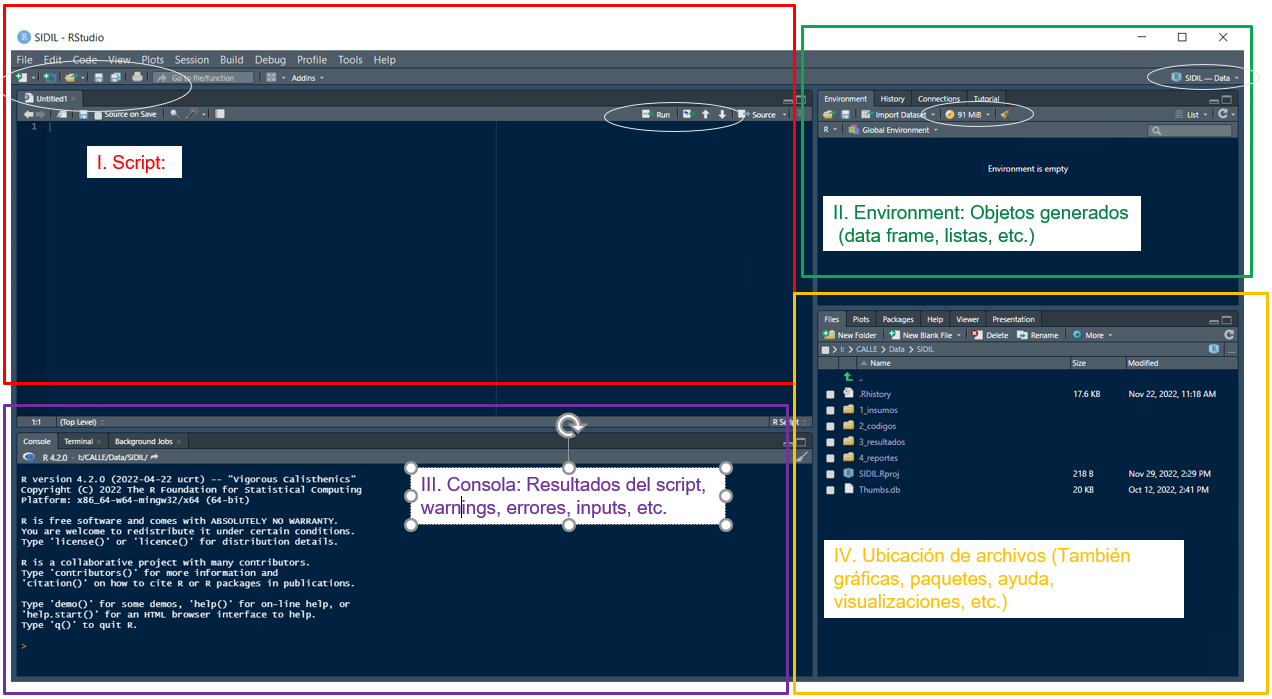
\includegraphics[width=17.67in]{images-1/06/RStudio} \caption{Entorno de RStudio}\label{fig:entornoRStudio}
\end{figure}

\hypertarget{procedimiento-para-ejecutar-proyectos-y-scripts-en-rstudio}{%
\subsection{Procedimiento para ejecutar proyectos y scripts en RStudio}\label{procedimiento-para-ejecutar-proyectos-y-scripts-en-rstudio}}

Abrir el proyecto SIDIL: Esto es fundamental, porque los proyectos en R Studio mantienen de manera ordenada en una misma ruta todos los elementos necesarios para que los códigos se ejecuten de manera correcta, de igual manera albergan los resultados que se producen de dichos códigos.

Lo importante es primero abrir el proyecto SIDIL, sea desde el Explorador de Windows o desde RStudio.

\begin{itemize}
\item
  Si se abre desde el explorador de archivos, se podrá identificar el proyecto por el logo de R y por el tipo de archivo .Rproj. Si se ha abierto con anterioridad el proyecto, este podría desplegar los scripts que se hayan utilizado con anteriormente, si no, será necesario abrir los scripts que se deseen ejecutar o editar en la primera sección de la pantalla (I. Scripts) o seleccionándolos directamente en la sección IV de ubicación de archivos.
\item
  Si se abre desde el programa RStudio, primero se debe asegurar que no esté ningún proyecto cargado. En la parte superior derecha (sección II de la pantalla), se puede identificar el proyecto en el que se está trabajando. En la ilustración \ref{fig:RStudioProyectoVacio} se observa que en el ambiente no se muestra ningún proyecto. Al hacer clic sobre la flecha señalando hacia abajo se despliega el menú que permite seleccionar ``Open Project\ldots{}'' (ilustración \ref{fig:RStudioOpenProject}) , navegar hasta la ubicación del proyecto \emph{SIDIL.Rproj} seleccionarlo y abrirlo para.
\end{itemize}

\begin{figure}
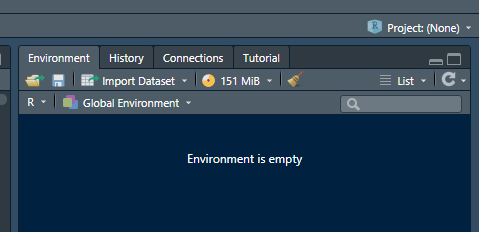
\includegraphics[width=6.65in]{images-1/06/proyectoVacio} \caption{Vista del ambiente sin proyecto}\label{fig:RStudioProyectoVacio}
\end{figure}

\begin{figure}
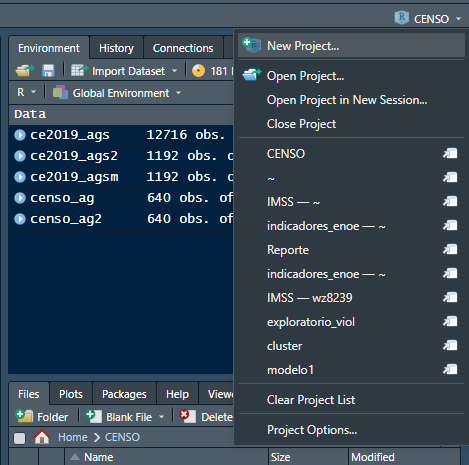
\includegraphics[width=6.51in]{images-1/06/openproject} \caption{Vista del ambiente sin proyecto}\label{fig:RStudioOpenProject}
\end{figure}

Si hubiera algún proyecto previamente cargado, se debe cerrar desplegando el menú del proyecto y seleccionando ``Close Project'' (tercera opción en la ilustración \ref{fig:RStudioOpenProject}).

El siguiente paso es abrir el script que se desea correr o editar, o bien, generar un nuevo script: Los archivos de códigos que utiliza el proyecto SIDIL en el ambiente RStudio puede ser de dos tipos: R Script (tipo. R) o R Markdown (tipo .Rmd). Para abrir un archivo ya existente o generar uno nuevo se puede realizar desde la primera sección de la pantalla (I. Scripts), donde el primer ícono despliega las opciones de nuevos documentos que se quieren creen, y el tercero abre el explorador de archivos para seleccionar alguno de los documentos ya existentes. Un script ya existente también se puede abrir desde la sección IV del programa RStudio, únicamente hace clic sobre el archivo. R o .Rmd que se desee abrir.

Una parte primordial para la ejecución de los scripts es la instalación y el llamado de las paqueterías que se utilizarán, ya que estas albergan los comandos que se utilizan en los archivos de códigos. Si bien R Studio cuenta con algunos comandos básicos, la versatilidad del programa permite importar y utilizar cientos de paqueterías que facilitan la generación de códigos con sus comandos. A continuación, se presentan las paqueterías que utiliza el proyecto SIDIL junto con algunos de los principales comandos de cada una. Esta lista de principales comandos no es exhaustiva y muchas paqueterías pueden contener cientos de comandos.

\begin{longtable}[]{@{}
  >{\raggedright\arraybackslash}p{(\columnwidth - 4\tabcolsep) * \real{0.0496}}
  >{\raggedright\arraybackslash}p{(\columnwidth - 4\tabcolsep) * \real{0.3588}}
  >{\raggedright\arraybackslash}p{(\columnwidth - 4\tabcolsep) * \real{0.5878}}@{}}
\caption{Tabla XXX: Principales paquetes usados en R.}\tabularnewline
\toprule\noalign{}
\begin{minipage}[b]{\linewidth}\raggedright
Paquete
\end{minipage} & \begin{minipage}[b]{\linewidth}\raggedright
Principal función
\end{minipage} & \begin{minipage}[b]{\linewidth}\raggedright
Principales comandos
\end{minipage} \\
\midrule\noalign{}
\endfirsthead
\toprule\noalign{}
\begin{minipage}[b]{\linewidth}\raggedright
Paquete
\end{minipage} & \begin{minipage}[b]{\linewidth}\raggedright
Principal función
\end{minipage} & \begin{minipage}[b]{\linewidth}\raggedright
Principales comandos
\end{minipage} \\
\midrule\noalign{}
\endhead
\bottomrule\noalign{}
\endlastfoot
pacman & Instalar y llamar paqueterías & p\_load() \\
here & Establecer el directorio en el que se trabaja & here () \\
tidyverse & Colección de paqueterías de gramática, estructura de datos, gráficas, entre otras. & operador pipe ``\%\textgreater\%'' , read\_csv(), filter(), group\_by(), mutate(), rename(), summarise(), str\_detect() (y otros str\_), as\_tibble (), pivo()t, gather() \\
haven & Lee archivos sav, dta, entre otros & read\_sav(), read\_dta() \\
dbplyr & Permite trabajar con bases de datos de distinto tipo & show\_query(), collect() \\
foreign & Permite leer y guardar archivos de distinto tipo & read.dbf () \\
janitor & Paquetería de gramática y estructura de datos & clean\_names(), tabyl() \\
readxl & Lee archivos de Excel & read\_excel() \\
survey & Paquetería para encuestas complejas & svymean(), svyby() \\
srvyr & Paquetería para encuestas complejas, agrega la sintaxis de tidyverse a la paquetería survey & as\_survey\_design(), survey\_mean(), survey\_total() \\
surveycv & Paquetería para encuestas complejas, permite cálculo de coeficiente de variación & cv.svy() \\
tidymodels & Colección de paqueterías para modelaje y machine learning utilizando el lenguaje tidyverse & Rsample (),training(), prep() \\
crayon & Cambia el color de los mensajes de la consola & styles(), crayon() \\
data.table & Herramientas para el manejo de objetos de bases de datos & fread(), file.exists() \\
stats & Paquetería para cálculos y herramientas estadísticas & gl(), glm(), \\
scriptName & Recupera nombres y ubicación de scripts & current\_filename() \\
rstudioapi & Accede a Rstudio API si está disponible & isavailable() \\
stringi & Paquetería para procesamiento de lenguaje natural & stri\_extract\_all(),

str\_detect(), \\
beepr & Genera sonidos de notificación & beep() \\
rlang & Funciones esenciales para el funcionamiento de Rstudio & Diversos elementos de funcionamiento interno. \\
tools & Funciones esenciales para el funcionamiento de Rstudio & Diversos elementos de funcionamiento interno. \\
\end{longtable}

Existen algunos comandos que se usan con más frecuencia y que resultan muy importantes para la lectura y procesamiento de la información. Algunos de estos son:

\begin{itemize}
\tightlist
\item
  Comandos read\_excel() y read\_csv(): Estos comandos permite leer y cargar archivos de formato .xlsx y .csv al ambiente de RStudio. Ejemplo:
\end{itemize}

\emph{correspondencia\_cat\_scianHOGARES\textless-read\_excel(``I:/CALLE/Data/SIDIL/1\_insumos/catálogos/clasificacion\_industrialcat\_scianHOGARES.xlsx'')}

Notar que en Rstudio los separadores diagonales o slash deben estar inclinados a la derecha (/).

\begin{itemize}
\tightlist
\item
  El comando here(): permite establecer la ruta donde se ejecutarán los archivos, suele ser la misma donde se localiza el proyecto R. Es muy útil para cargar y guardar archivos, ya que únicamente se tendrá que utilizar el comando here() para reemplazar toda la ruta, que de otra manera tendría que ser escrita en su totalidad. Ejemplo:
\end{itemize}

\begin{quote}
\emph{correspondencia\_cat\_scianHOGARES\textless-read\_excel(here(), ``1\_insumos'',``catálogos'',``clasificacion\_industrial'',``cat\_scianHOGARES.xlsx'')}
\end{quote}

\begin{itemize}
\tightlist
\item
  Los comandos paste() y paste0(): Estos comandos funcionan para concatenar elementos. El primero permite determinar un separador entre los elementos. Ejemplo:
\end{itemize}

\emph{bitacora \textless- read\_csv(paste(here(),``4\_reportes'',``bitacoras'',``bitacora.csv'',sep = ``/'')}

\begin{itemize}
\tightlist
\item
  El comando source(): Este comando permite llamar y correr otros archivos script .R y .Rmd desde otro script. En otras palabras, el comando facilita la ejecución de múltiples scripts desde uno solo. Ejemplo:
\end{itemize}

\emph{source(here(``2\_codigos'',``cod\_config\_inicial'',``0\_config\_inicial.R''))}

\begin{itemize}
\tightlist
\item
  El operador pipe '' \%\textgreater\% ``: este operador permite concatenar diversas líneas de código sobre un mismo objeto, sin necesidad de volverlo a''llamar'' o nombrar. Ejemplo:
\end{itemize}

\emph{enoe \textless- ENOEN\_sdemycoes \%\textgreater\% mutate(contrato\_escrito=ifelse(contrato\_escrito==1,1,0))}

\begin{itemize}
\tightlist
\item
  Los comandos \_join: comprende left\_join(), right\_join(), full\_join(), semi\_join(), inner\_join() y anti\_join(). Este grupo de comandos se utiliza para unir dos data frames o tablas. Ejemplo:
\end{itemize}

\emph{ENOEN\_sdemycoes \textless-left\_join(ENOEN\_sdemycoes, correspondencia\_cat\_scianHOGARES, by=c(``p4a\_tres''=``scian\_hogares\_2018'')}

\begin{itemize}
\tightlist
\item
  El comando mutate(): sirve para crear nuevas variables o campos dentro de un data frame o tabla, es muy importante para la transformación de la información. Ejemplo:
\end{itemize}

\emph{enoe \textless- ENOEN\_sdemycoes \%\textgreater\% mutate(ing\_min=ifelse(ing7c==1,1,0))}

\begin{itemize}
\tightlist
\item
  El comando filter(): permite filtrar información de una variable o campo excluyendo una o muchas de sus categorías o rangos. Ejemplo:
\end{itemize}

\emph{ENOEN\_sdemycoes \textless- ENOEN\_sdemycoes \%\textgreater\% filter(p3h==1)}

\begin{itemize}
\tightlist
\item
  El comando select(): selecciona una o más variables o campos de un data frame o tabla. Ejemplo:
\end{itemize}

\emph{ENOEN\_sdemycoes \textless- ENOEN\_sdemycoes \%\textgreater\% filter(p3h==1)}

\begin{itemize}
\tightlist
\item
  El comando select(): selecciona una o más variables o campos de un data frame o tabla. Ejemplo:
\end{itemize}

\emph{ENOEN\_sdemycoes \textless- ENOEN\_sdemycoes \%\textgreater\% filter(p3h==1)}

\begin{itemize}
\tightlist
\item
  El comando case\_when(): funciona para clasificar o reclasificar categorías de una variable o campo (cuando a, entonces b; cuando c, entonces (simbolizado por '' \textasciitilde{} ``) d; etc.). Este comando permite hacer comparaciones entre categorías de la misma variable o entre diferentes variables utilizando símbolos de igualdad y desigualdad como''=``,''\textgreater{}``,''\textless{}``,''!='' (diferente) para crear las nuevas categorías. Ejemplo:
\end{itemize}

\emph{ENOEN\_sdemycoes\textless-ENOEN\_sdemycoes \%\textgreater\% mutate(cat\_tamanio= as.factor(case\_when(}

\emph{cat\_tamanio\textless=3\textasciitilde{}`1', cat\_tamanio==4\textasciitilde{}`2', cat\_tamanio\textgreater=5 \& cat\_tamanio\textless=7\textasciitilde{}`3', cat\_tamanio==8\textasciitilde{}`4', cat\_tamanio==9\textasciitilde{}`5', cat\_tamanio\textgreater=10\textasciitilde{}`6')))}

Notar que el case\_when clasifica las situaciones con la jerarquía con la que sucede la ocurrencia: Es decir, si una observación cumple con dos ``casos'' entonces al evaluarse el primer caso y cumplirse, ya no se evalúa el segundo caso.

\begin{itemize}
\item
  El comando if\_else() o ifelse(): Al igual que el comando anterior, funciona para reclasificar categorías de variables o campos, aunque esta función permite solo dos opciones de clasificación (si sucede x, entonces y). Ejemplo:\\
  \emph{enoe \textless- ENOEN\_sdemycoes \%\textgreater\% mutate(presta\_soc=ifelse(pre\_asa==1,1,0))}
\item
  El comando for(): Este comando permite hacer iteraciones de uno o más comandos sobre los elementos declarados, estos elementos pueden ser pertenecientes a un vector o lista. Ejemplo:\\
  \emph{for (i in lista\_indicadores\_enoe)\{}\\
  \emph{dir.create(paste0(here(``3\_resultados/coyuntura/res\_coy\_ENOE'', i)))}\\
  \emph{ENOE'')) \}}
\item
  Comandos sub(), gsub(), y aquellos que inician con stri\_() o str\_(): Estos comandos sirven para transformar e identificar patrones en cadenas de texto (o procesamiento de lenguaje natural) utilizando diversos códigos. Ejemplo:\\
  \emph{filter(str\_detect(nombre\_archivo,``SDEM''))}
\item
  Comando as\_survey\_design(): este comando se utiliza para declarar una base de datos como encuesta a partir de sus variables muestrales. Ejemplo:\\
  \emph{enoesvyset \textless- enoe \%\textgreater\% as\_survey\_design(strata = estrato, weights = peso, id = upm, nest=TRUE)}
\item
  Comandos que empiezan con svy\_() o survey\_(): Estos comandos toman en cuenta la encuesta declarada para hacer cálculos sobre la misma considerando su diseño muestral. Entre estos podemos encontrar: survey\_mean() y survey\_ratio(). Estos comandos brindan la opción de obtener el error estándar (se), los intervalos de confianza (ci), la varianza (var), y los coeficientes de variación (vi) de las estimaciones calculadas. Ejemplo:\\
  \emph{valor=survey\_mean(ing\_min, vartype = c(``cv''), na.rm=T)}
\item
  Comando try\_catch(): Este comando permite poner condiciones a la ejecución de otros comandos en R. Suele utilizarse para mostrar errores y warnigs que se deben tener en cuenta, por ejemplo, si no se encontró algún archivo o script. Usualmente el comando impide que se detenga la ejecución del código ante posibles errores, aunque se debe prestar especial atención a los mensajes de error y warnings que se produzcan en la consola. Ejemplo:\\
  \emph{municipios\_frontera\_norte \textless-tryCatch(suppressMessages(read\_csv(} \emph{paste(path\_a\_marco\_geo,``municipios\_fn'',``municipiosFronteraNorte.csv'',sep=``/''),error= function(e) \{cat(crayon::red(``\textbackslash n'',``\textbackslash n'',paste(``*** ERROR *** No se ha cargado: Catalogo de municipios en la frontera norte.'')),``\textbackslash n'',``\textbackslash n'')\})}
\item
  Comando saveRDS(): este comando permite guardar data frames en formato .Rds. Ejemplo: \emph{saveRDS(enoe\_temp,paste0(here(),``/'', ``3\_resultados/coyuntura/res\_coy\_ENOE'',``/'' ,nombre,``/enoe\_'',nombre,``\_'',periodo,anio,``\_'',v,``.Rds''))}\\
  \strut \\
  Existen otros comandos para guardar las bases de datos en otros formatos: write.csv(), write.dta(), entre otros.
\end{itemize}

Además de estos, se utilizan muchos otros comandos de las paqueterías cargadas, no obstante, estos son los que se utilizan con más frecuencia ya que son los básicos para la carga, transformación y guardado de la información que utiliza el SIDIL. Si surge alguna duda, o si se requiere profundizar en estos u otros comandos, existe amplia información en internet que incluye explicaciones y ejemplos sobre el uso de los diversos comandos en el ambiente de RStudio, dos de las principales fuentes de consulta son: www. cran.r-project.org y \href{http://www.stackoverflow.com}{www.stackoverflow.com}, o bien con el comando help(package=``\_\_''), poniendo entre las comillas el nombre de la paquetería que se desea buscar. De igual manera, si se desea buscar información sobre algún comando, se puede utilizar la línea de código help(\_\_, package=``\_\_''), poniendo en el primer argumento el comando en cuestión y en el segundo la paquetería al que pertenece.

\hypertarget{tipos-de-errores-que-se-pudieran-presentar}{%
\subsection{Tipos de errores que se pudieran presentar}\label{tipos-de-errores-que-se-pudieran-presentar}}

Típicamente se pueden presentar los siguientes errores al trabajar en RStudio.

\begin{enumerate}
\def\labelenumi{\arabic{enumi})}
\item
  Errores de lectura de información

  \begin{enumerate}
  \def\labelenumii{\alph{enumii}.}
  \item
    Ubicación de los archivos mal escrito: este suele el error más frecuente para la lectura de archivos. Se debe asegurar que la ubicación y el nombre de los archivos se escriba correctamente para su optima apertura.
  \item
    Tipo de archivos: De igual manera, se debe asegurar que se esté utilizando el comando correcto para cada tipo de archivo. Es decir, si se quiere abrir un archivo .csv se debe utilizar el comando ``read\_csv'', mientras que si se quiere abrir un archivo .Rds se debe utilizar el comando ``readRDS''.
  \end{enumerate}
\item
  Errores de procesamiento de información

  \begin{enumerate}
  \def\labelenumii{\alph{enumii}.}
  \item
    Problemas con los campos

    \begin{enumerate}
    \def\labelenumiii{\roman{enumiii}.}
    \item
      Campos que no se encuentran: Este error puede estar relacionado con problemas de cambio de los nombres de los campos o que directamente se dejaron de incluir por diversas razones en la fuente de información original
    \item
      Problemas con el tipo de variables o campos del data frame: No todas las transformaciones se pueden hacer a todos los tipos de variables o campos, es por esto por lo que primero se debe asegurar que el campo a transformar sea el que deseamos. Para esto, se puede utilizar el comando class(dataframe\$campo). Para realizar un cambio en el tipo de un campo se pueden utilizar los comandos que inician as.\_(), por ejemplo: as.double(dataframe\$campo), as.character(dataframe\$campo), entre otros.
    \end{enumerate}
  \item
    Insuficiencia de memoria RAM para el procesamiento

    \begin{enumerate}
    \def\labelenumiii{\roman{enumiii}.}
    \item
      Este es un error que reporta directamente el RStudio con el mensaje \emph{``cannot allocate vector\ldots.''}

      \begin{enumerate}
      \def\labelenumiv{\arabic{enumiv}.}
      \item
        Hay dos posibles causas:

        \begin{enumerate}
        \def\labelenumv{\alph{enumv}.}
        \tightlist
        \item
          Que en efecto el procesamiento de la información sea el adecuado, pero quizá, incluso por otros procesos en curso, la computadora no cuenta con la memoria suficiente. Para esto se deben finalizar en el administrador de tareas los programas que no estén en uso, y desde la consola de RStudio, desplegar el menú de memoria en uso del ambiente, y liberal memoria que no esté en uso, como muesta la ilustración \ref{fig:memoriaRstudio}.
        \end{enumerate}
      \end{enumerate}
    \end{enumerate}
  \end{enumerate}
\end{enumerate}

\begin{figure}
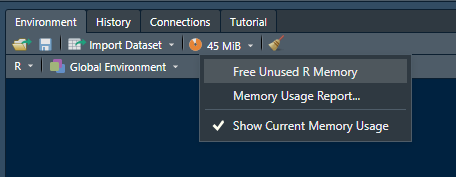
\includegraphics[width=6.33in]{images-1/06/memoriaR} \caption{Liberación de memoria en RStudio}\label{fig:memoriaRstudio}
\end{figure}

\begin{enumerate}
\def\labelenumi{\alph{enumi}.}
\setcounter{enumi}{1}
\tightlist
\item
  Que el algoritmo no esté procesando la información en la estructura predefinida lo que genera objetos cuyas dimensiones no son las correctas y consumen excesiva memoria. Por ejemplo, duplicidades innecesarias en algunos registros que se pretenden unir entre diferentes bases con la misma información.
\end{enumerate}

\begin{quote}
Si el error es debido a lo anterior, se debe asegurar que los insumos utilizados en los procedimientos sean los correctos.
\end{quote}

\begin{enumerate}
\def\labelenumi{\arabic{enumi})}
\setcounter{enumi}{2}
\item
  De error en el lenguaje:

  \begin{enumerate}
  \def\labelenumii{\roman{enumii}.}
  \item
    Mal escrito el código: Es muy frecuente que los errores se den porque, al insertar líneas de códigos hay algún error de tipeo.
  \item
    La paquetería ya no incluye el comando sugerido

    \begin{enumerate}
    \def\labelenumiii{\arabic{enumiii}.}
    \item
      Pudiera ser un warning, que desde CRAN no se informa la falta de mantenimiento/seguimiento a dicho comando/paquete. Esta advertencia no detendrá el proceso, pero se debe hacer seguimiento a dicho comando en caso de que se deje de incluir definitivamente
    \item
      Podría ser un error en el cual, por diversos motivos, ya no se incluye el comando en la paquetería seleccionada. Usualmente cuando esto sucede la propia consola de R muestra los nuevos códigos con los que fue reemplazado el código en desuso
    \end{enumerate}
  \end{enumerate}
\end{enumerate}

La consola de RStudio siempre mostrará el error y alguna información extra, esta debe ser tenida en cuenta ya que muestra la naturaleza del error y, algunas veces, la solución, de no ser así, se puede rastrear el error y solucionarlo con ayuda de internet.

\hypertarget{python}{%
\subsection{Python}\label{python}}

A continuación, se dará una breve descripción de las principales librerías de Python usadas para el SIDIL. Entre paréntesis se indica el número de versión que se utiliza de cada librería.

\begin{itemize}
\item
  Numpy (1.23.4) proporciona soporte para el cálculo numérico y la manipulación de datos en forma de arrays y matrices. Es muy útil para realizar cálculos matemáticos y estadísticos de forma eficiente, y es una de las librerías más utilizadas en el área de la ciencia de datos.
\item
  Pandas (1.4.4) se utiliza para la manipulación y análisis de datos. Ofrece una serie de herramientas para importar, limpiar, transformar y visualizar datos de forma sencilla y rápida. Es muy útil para el procesamiento y análisis de conjuntos de datos de gran tamaño y complejidad.
\item
  Scikit-learn (1.1.2) proporciona una amplia gama de algoritmos de aprendizaje automático y herramientas para el análisis de datos. Incluye una gran variedad de modelos de aprendizaje automático, como árboles de decisión, regresión lineal y SVM, y proporciona una interfaz sencilla y consistente para su uso.
\item
  PyTorch (1.12.1) para el desarrollo de redes neuronales y aprendizaje automático profundo. Ofrece una amplia gama de herramientas y funcionalidades para el diseño y entrenamiento de modelos de aprendizaje automático profundo (\emph{Deep} \emph{learning}). Además esta librería permite acceder al modelo tabnet que es la primera variante al modelo Random forest que resultó ser el esocigod tcon base en las métricas de performance.
\item
  Matplotlib (3.6.2): se utiliza para crear gráficos y visualizaciones interactivas de datos en 2D y 3D. Matplotlib ofrece una amplia variedad de tipos de gráficos, como líneas, barras, histogramas, dispersión, gráficos de torta, entre otros.
\item
  Yellowbrick (1.5): se enfoca en la visualización y diagnóstico de modelos de aprendizaje automático. Proporciona una variedad de gráficos y herramientas interactivas para evaluar y entender el rendimiento y el comportamiento de los modelos de aprendizaje automático. Es una herramienta útil para el análisis y mejora de modelos, lo que ayuda a tomar decisiones más informadas en el proceso de desarrollo de algoritmos de aprendizaje automático.
\item
  Pydotplus (2.0.2): se utiliza para la generación y visualización de gráficos de redes y árboles en Python. Se utiliza principalmente para visualizar estructuras de datos jerárquicas, como árboles de decisión generados por algoritmos de aprendizaje automático.
\item
  Clean-text (0.6.0): se utiliza en la limpieza y preprocesamiento de datos de texto. Proporciona una variedad de funciones para eliminar caracteres especiales, eliminar stopwords, realizar lematización y más.
\item
  Pyreadr (0.4.7): es una librería para facilitar la lectura y escritura de archivos en diversos formatos, como CSV, Excel y más. Proporciona funciones para cargar y guardar datos en diferentes formatos, lo que simplifica la manipulación de conjuntos de datos almacenados en archivos externos.
\item
  Shap (SHapley Additive exPlanations, 0.41.0): se utiliza para explicar las predicciones de modelos de aprendizaje automático. Se basa en la teoría de juegos y proporciona un marco de trabajo para calcular la importancia de cada característica (atributo) en el resultado de un modelo. Shap es una herramienta útil para interpretar y entender el comportamiento de modelos de aprendizaje automático, lo que puede ayudar a aumentar la confianza en sus predicciones y detectar posibles sesgos.
\end{itemize}

\hypertarget{especificaciones-del-servidor}{%
\section{Especificaciones del servidor}\label{especificaciones-del-servidor}}

PENDIENTE PEGAR

\hypertarget{conceptos-y-hallazgos-clave-en-la-exploraciuxf3n-del-siapi-sipas}{%
\section{Conceptos y hallazgos clave en la exploración del SIAPI-SIPAS}\label{conceptos-y-hallazgos-clave-en-la-exploraciuxf3n-del-siapi-sipas}}

Esta sección presenta el análisis que AIR hizo sobre los sistemas con los que cuenta la STPS para el apoyo a la inspección laboral (SIAPI) y al proceso sancionador (SIPAS), con dos principales propósitos. Primero, profundizar en algunos de los conceptos que resultan críticos en la explotación de los registros administrativos de la inspección. Esto para homologar un único vocabulario e interpretación del alcance del SIDIL en lo que refiere a la inspecciones; segundo, para dar cuenta del volumen de información y la calidad de la misma y que el SIDIL consume a efectos de realizar las predicciones.

La sección está organizada de la siguiente manera:

\hypertarget{conceptos-y-clasificaciones-relevantes.}{%
\subsection{Conceptos y clasificaciones relevantes.}\label{conceptos-y-clasificaciones-relevantes.}}

Conviene comenzar por la importancia de la explotación de los registros administativos. Quizá la principal información que interesa extraerse del SIAPI es si la inspección ha detectado violaciones a la normativa laboral porque es, justamente, lo que el modelo busca predecir. \textbf{La variable dependiente que entra en el entrenamiento del modelo predictivo será aquel aspecto para el cual luego el modelo, al aplicarlo, buscará predecir su ocurrencia.} Seleccionar otra información como variable dependiente, implicará que el modelo prediga sobre esa otra información de entrada.

\textbf{Como se ha mencionado al explicar el \protect\hyperlink{procesamientoModIVSIAPI}{entrenamiento} del modelo, éste toma como variable dependiente la detección de violaciones que proceden, una vez que las inspecciones son calificadas por la \hl{UTD} y se acepta como procedente para iniciar el procedimiento de sanción}. Pues bien, este anexo guia a el / la lector/a a identificar cómo es que se arriba a esta definición y cómo se mide, para lo cual el recorrido no es del todo lineal ni evidente para aquellas personas menos familiarizadas con el sistema. \textbf{Notar que, mientras que la explotación de los registros administrativos obedece fundamentalmente a la necesidad de \emph{entrenar} el modelo a partir de los centros de trabajo que fueron inspeccionados, la predicción del mismo, se realiza sobre el universo total de los mismos, independientemente de su historial de inspecciones.}

Una importante precisión es que en la STPS los sistemas de apoyo a la inspección han tenido a lo largo de los años diferentes ``instancias'' o ``cortes'', que se condicen con cada uno de los cambios importantes en la normatividad de la inspección. Esto se debe a que las herramientas utilizadas para apoyar los procesos de inspección no contaban hasta ahora con mecanismos que permitan el manejo y administración de diferentes versiones del marco normativo en una sola instancia del sistema. Por lo cual, ante un nuevo reglamento de inspección o ante una modificación sustantiva a la las leyes y normas en la materia, se requirió copiar el sistema en una nueva instancia en la cual se pudieran reflejar la situación normativa derivada de esa modificación.\footnote{Como parte de su colaboración con STPS, AIR ha desarrollado un gestor de normativ}

Son cinco los ``cortes'' que se han realizado a la base de datos, mismos que se han integrado para realizar el análisis que se presenta a continuación. Los 5 ``cortes'' representan la totalidad de la base de datos y la integración selectiva de los diferentes casos (inspecciones) a lo largo de los diferentes ``cortes'' previene de duplicar la información y la tergiversación de los hallazgos, se ha requerido un importante trabajo de análisis para la unificación de bases de datos y generar el universo global de las inspecciones realizadas. Esta tarea requirió por supuesto entender la lógica en que se debe hacer la agregación de las inspecciones y ha dado como resultado un universo de cerca de un millón cien mil inspecciones totales en el período, conformándose así el universo de análisis. Cabe agregar que, por lo general, con los diferentes cortes que se realizan se generan pequeños cambios en las taxonomías de algunas variables, y, en menor medida, surgen nuevas tablas al interior de la base de datos.

El volumen de información que se encuentra en cada uno de los ``cortes'' varía, y como se observa en la ilustración \ref{fig:volumeninspecciones}, de los cinco ``cortes'' distintos que se realizaron a la base de datos, el primero consta de cerca de 60 mil inspecciones, con inspecciones que se realizaron entre junio 2012 y abril 2015, mientras que el último corte es el que incorpora las inspecciones realizadas entre enero 2020 y octubre 2021.

\begin{figure}
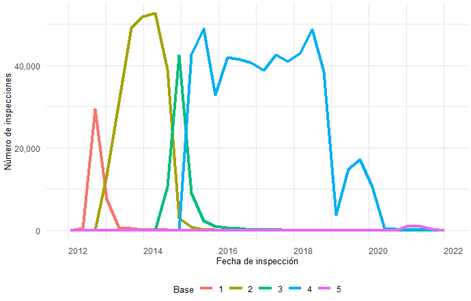
\includegraphics[width=6.54in]{images-1/08/volumeninspecciones} \caption{Módulos que componen el SIDIL}\label{fig:volumeninspecciones}
\end{figure}

Recuadro \hl{xx1}: Conformación del \emph{índice} de inspecciones

\begin{longtable}[]{@{}
  >{\raggedright\arraybackslash}p{(\columnwidth - 0\tabcolsep) * \real{1.0010}}@{}}
\toprule\noalign{}
\begin{minipage}[b]{\linewidth}\raggedright
La existencia de múltiples instancias de la base de datos del SIAPI obliga a conformar un índice de inspecciones para evitar su conteo duplicado. La lógica es que, de no hacerlo, una misma inspección podría incorporarse hasta 5 veces en la base de entrenamiento.

A tal efecto, el algoritmo \emph{4\_query\_violaciones\_inspecciones\_} realiza en un primer momento una explotación de todos los campos \emph{inspeccion\_id} de todas las instancias del SIAPI. De cada instancia recupera todas las inspecciones que ésta contenga. Acto seguido, identifica para cada inspección la primera instancia en la que \emph{aparece} esta inspección. Ésta será la instancia a la que se asociará la inspección. En todas las consultas y emparejamientos subsecuentes se buscará únicamente la información sobre la inspección que haya sido registrada en dicha instancia. De haber información que erroneamente se haya registrado sobre la inspección en otra instancia, ésta no será tomada en cuenta. La lógica detrás, validada con la UTD, es que el marco normativo con el que nace la inspección es el que se mantendrá vigente a lo largo de todo el proceso inspectivo, motivo por el cual, toda información que se genera en las diversas etapas del procedimiento serán recuperadas de esa instancia donde por primera vez \emph{nace´} la inspección, únicamente.
\end{minipage} \\
\midrule\noalign{}
\endhead
\bottomrule\noalign{}
\endlastfoot
 \\
\end{longtable}

Dada la posibilidad de la coexistencia de diferentes marcos normativos (ver recuadro \hl{XXX 1 XX}) existe una intersección temporal entre los diferentes ``cortes'', explicando además que el volumen de inspecciones que representa el ``corte'' 4, mismo que va de diciembre 2012 a septiembre 2021, represente al 56\% de las inspecciones registradas, como se observa en la tabla \hl{xxx1xxx} Ambos aspectos se explican por la misma causa: los ``cortes'' representan cambios al marco normativo, mientras que cada proceso de inspección debe por lógica corresponder con un único marco normativo (la inspección que ``nace'' bajo un marco normativo se sostiene en ese ámbito, incluso cuando éste marco jurídico es reemplazado por uno nuevo). Por ello mientras se va concluyendo el proceso inspectivo de un caso, es posible que ante un nuevo cambio normativo coexistan temporalmente diferentes versiones del sistema.

Tabla xxx1xxx. Distribución de las inspecciones, por fecha de inspección y ``corte'' de la base.
\hl{PENDIENTE hacer tabla}
Corte de la base Fecha inicial Fecha final Número de inspecciones
1 15/08/2012 27/11/2012 59,879
2 23/04/2013 05/08/2014 318,772
3 09/10/2014 12/03/2015 115,109
4 03/07/2015 14/11/2018 633,176
5 28/01/2021 31/07/2021 2,794
Total 1,129,730

\textbf{Fuente: Elaboración propia a partir del SIAPI-SIPAS. Nota: las fechas iniciales y fecha finales comprenden al decil 1 y al decil 9, respectivamente de cada base de datos, es decir, pueden encontrarse fechas anteriores y posteriores a las indicadas, pero son excepciones. }

\hypertarget{planeaciuxf3n-de-la-inspecciuxf3n}{%
\subsubsection{Planeación de la inspección}\label{planeaciuxf3n-de-la-inspecciuxf3n}}

Si bien el SIDIL es una herramienta estratégica para la programación de inspecciones en el marco de operativos de inspección (por definición, son inspecciones del \emph{tipo} \emph{extraordinario}), la información que se explota para el entrenamiento del modelo no se limita a este tipo de inspecciones.

La planeación del año se realiza conforme a la disponibilidad de recursos y las prioridades de política pública. Por lo general, a finales de cada año se realiza una planeación anual de las inspecciones para determinar las metas anuales para el año fiscal siguiente, conforme a la disponibilidad de inspectores por oficina, tomando además en cuenta las prioridades de política pública de la gestión. En promedio, entre 2012 y 2021 se estableció una meta anual de 91,026 inspecciones por año. A grandes rasgos se observan tres fases distintas en cuanto a este promedio, como se presenta en la ilustración \ref{fig:Metasanualesinspeccion}: entre 2012 y 2013, la meta anual osciló entre 86,000 y 89,000 inspecciones anuales; de 2014 a 2017 se ubicó entre 119,000 y 124,000 seguido por un máximo observado en 2018 con 130,000 inspecciones y de 2019 en adelante, la meta se redujo a la mitad e incluso hasta un tercio de los niveles de 2012 y 2013. En 2019 la meta alcanzó las 45,061 inspecciones, en 2020 las 30,721 inspecciones y en 2021 39,198 inspecciones. Como se observará más adelante, hay una discrepancia entre la meta anual y lo realizado de hecho, motivo por lo cual sería precipitado concluir en una reducción del volumen de la carga de trabajo.

La meta anual de inspecciones se distribuye en dos grandes tipos: las de programación aleatoria y las de programación directa. La programación aleatoria es la que se asocia con inspecciones del tipo ordinario, mientras que las de programación directa corresponde a las inspecciones del tipo extraordinario. Se suma un tercer tipo que es el de programación automática y que abarca las inspecciones de comprobación de medidas, como se explicará más adelante.

El conjunto de las inspecciones de programación aleatoria se compone de inspecciones iniciales y periódicas. Mientras que las inspecciones iniciales son las que se realizan por primera vez a un centro de trabajo (CT) o por ampliación o modificación de éstos , las periódicas tienen cierta frecuencia predeterminada según los resultados de las inspecciones anteriores realizadas al mismo CT, ``tomando en consideración la rama industrial, la naturaleza de las actividades que realicen, su grado de riesgo, número de trabajadores y ubicación geográfica'' . Ambas conforman buena parte de las inspecciones del tipo ordinaria, sumándose a este grupo las inspecciones de comprobación de medidas en materia de Seguridad e higiene, como se detalla más adelante.

Por su parte, las inspecciones de programación directa incluyen, pero no se limitan, a las inspecciones realizadas en el marco de un determinado operativo. Los operativos, como se verá más adelante, son un tipo de programación de inspección de un alcance específico que atiende a temáticas o prioridades predefinidas.
A lo largo de la década analizada el 54.9\% de las inspecciones realizadas fueron de programación directa, y el 45.1\% de programación aleatoria (ver ilustración 3). Esto no ocurrió sin cierta cierta variación de un año a otro: En 2018 fue cuando la programación directa tuvo el mayor peso (75\%), mientras que su menor participación fue en 2019, con tan sólo 20\% de la meta anual.

\begin{figure}
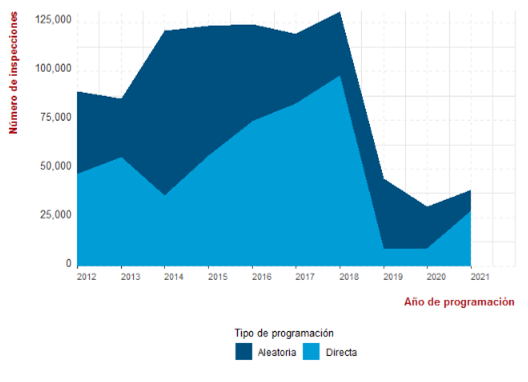
\includegraphics[width=7.33in]{images-1/08/Metasanualesinspeccion} \caption{Metas anuales de inspección, por tipo de inspección}\label{fig:Metasanualesinspeccion}
\end{figure}

\hypertarget{meta-y-realizaciuxf3n-de-inspecciones-a-realizar-por-tipo-estado-y-por-oficina}{%
\subsubsection{Meta y realización de inspecciones a realizar por tipo, estado y por oficina}\label{meta-y-realizaciuxf3n-de-inspecciones-a-realizar-por-tipo-estado-y-por-oficina}}

En el SIAPI se identificaron 109 oficinas responsables de las inspecciones o Unidades responsables (UR) distribuídas a lo largo de las 32 entidades federativas, sumándose 27 otras UR de carácter federal que corresponden a otras áreas de la STPS, como por ejemplo la DG de Inspección Federal del Trabajo, la DG de Asuntos Jurídicos, etc.. Las 109 UR típicamente toman la forma de una Oficina de Representación Federal del Trabajo (ORFT), de una Subdelegación Federal del Trabajo, de una Oficina Federal del Trabajo, de una Delegación Federal del Trabajo o de una Unidad Subalterna de la ORFT. Se asume que a efectos de la operación de las inspecciones como el seguimiento del proceso sancionador, no existen diferencias sustantivas en cuanto a las atribuciones que tiene cada una de ellas.

En promedio, en cada entidad federativa hay 3.4 UR, siendo Veracruz la entidad con mayor número de UR con 15 oficinas, y habiendo 17 entidades federativas con solamente 2 UR en su delimitación geográfica. Hay otras 14 entidades federativas que tienen entre 4 y 6 UR (\ref{fig:InspectoresUR}. El número de inspectores por cada UR varía entre 3 y 4 en Baja California Sur y Aguascalientes, respectivamente, y 49 y 87 en el Estado de México y la Ciudad de México. La ilustración da cuenta de la correlación positiva entre el número de centros de trabajo y el número de inspectores activos. Se observa que algunas entidades, como el Estado de México, Veracruz, Tamaulipas, presentan un número proporcionalmente menor de inspectores, mientras que Jalisco y Nuevo León superan la tendencia estatal.

\begin{figure}
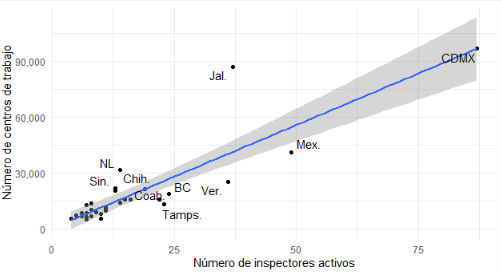
\includegraphics[width=6.97in]{images-1/08/InspectoresUR} \caption{Número de inspectores activos y CT cubiertos, por UR, a 2021.}\label{fig:InspectoresUR}
\end{figure}

La interacción entre la meta anual de inspecciones y el número de inspectores disponibles determina la carga de trabajo que se asigna a los inspectores. La planeación anual toma en consideración la disponibilidad de inspectores que se reporta a nivel descentralizado en cada una de las unidades responsables a través de las oficinas de representación, mismas que en su agregación conforman el total de número de inspectores disponibles. Sin embargo, a efectos de la programación de operativos, la disponibilidad de corto plazo de los inspectores no es algo que se pueda capturar en el sistema. \textbf{Es en este punto en donde el SIDIL, con la información disponible en el sistema, no puede incorporar de manera automatizada la disponibilidad de inspectores para la conformación de un universo de CT priorizados por riesgos (y atributos e indicadores) \emph{estratificado} o \emph{acotado} a la disponibilidad de inspectores en cada UR - toda vez que la información al respecto en el sistema no se actualiza en tiempo real.}

Establecida la meta anual de inspecciones se realiza su distribución a lo largo de tres dimensiones, la temporal, la geográfica y la temática o de alcance, de la siguiente manera: por un lado, la meta anual de inspecciones se distribuye en los doce meses del año (dimensión temporal), y a su vez, se le asigna el volumen a las oficinas que integran cada una de las entidades federativas (dimensión geográfica). Lo anterior aplica tanto para las inspecciones de programación aleatoria como de programación directa. por último, en cuanto a la temática, como se verá más adelante, se trata de la materia sustantiva sobre la que versará la inspección, que en el marco de este reporte se define como alcance, compuesto por materias, submaterias, indicadores e incisos, como se describe en la sección ``Alcance de la inspección'', más adelante y que se asigna, sólo en algunos de los casos, al momento de establecer las metas anuales.

Conviene aclarar, que a efectos de este reporte se define a una inspección como registrada, cuando ésta es programada y por lo tanto aparece en el sistema con un identificador único e intransferible, independientemente de la etapa o estatus en el que se encuentre esta inspección. Esta definición es importante, toda vez que más adelante se distinguirá entre inspecciones realizadas y no realizadas, siendo ambas parte de las inspecciones registradas.

Considerando la totalidad del país, se observa que la tendencia del número de inspecciones realizadas es superior al número de inspecciones programadas, pero sólo desde 2013 a 2018 inclusive. A partir de 2019 se registra un déficit en el número de inspecciones realizadas con respecto a la planeación anual, mismo que puede estar explicado por el cambio de administración a fines de 2018, como por la irrupción en México de la pandemia de COVID-19 en el año 2020. Complementando lo anterior, en la ilustración 9 se presenta la evolución mensual de ambas variables a lo largo de la década 2012-2021. Además de justificar la afirmación anterior, esta ilustración da cuenta de que ambas variables presentan una elevada volatilidad (cambios abruptos de un mes a otro) y ciclicidad (los meses de diciembre y enero son, por lo general, los de menor volumen).

\begin{figure}
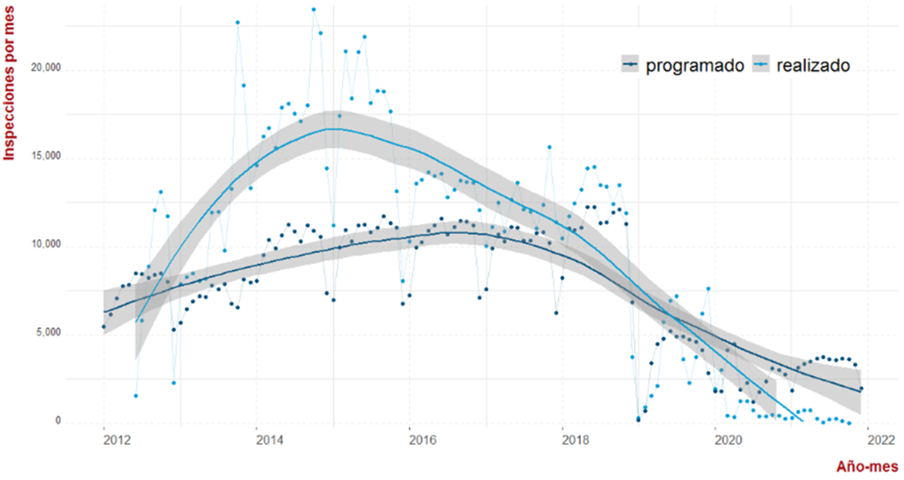
\includegraphics[width=12.56in]{images-1/08/programadorealizado} \caption{Módulos que componen el SIDIL}\label{fig:programadorealizado}
\end{figure}

\hypertarget{aspectos-pendientes-y-posibles-extensiones-a-futuro}{%
\subsection{Aspectos pendientes y posibles extensiones a futuro}\label{aspectos-pendientes-y-posibles-extensiones-a-futuro}}

\hypertarget{limitaciones-en-la-construcciuxf3n-de-la-variable-dependiente}{%
\subsubsection{Limitaciones en la construcción de la variable dependiente}\label{limitaciones-en-la-construcciuxf3n-de-la-variable-dependiente}}

\hypertarget{posibles-alternativas-como-variable-dependiente}{%
\subsubsection{Posibles alternativas como variable dependiente}\label{posibles-alternativas-como-variable-dependiente}}

\hypertarget{section}{%
\subsubsection{}\label{section}}

\hypertarget{box-and-tables}{%
\section{Box and tables}\label{box-and-tables}}

\begin{figure}
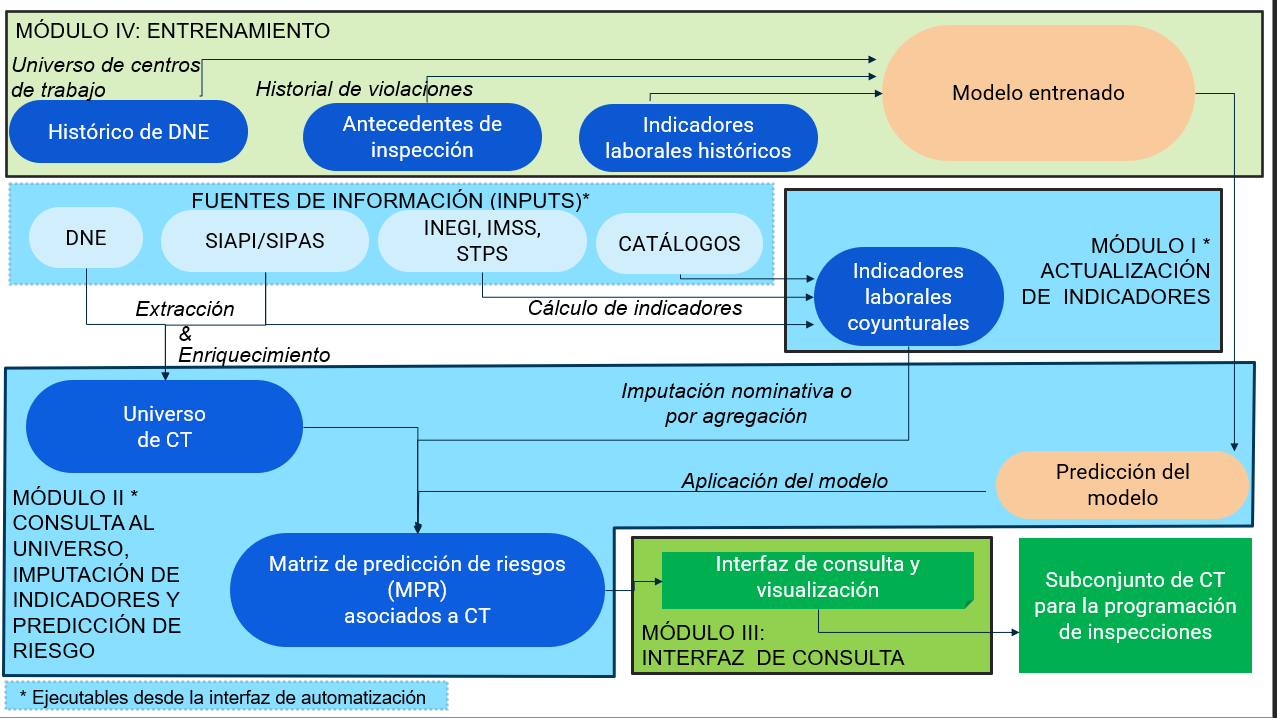
\includegraphics[width=17.74in]{images-1/02/pipeline_elaborado} \caption{Módulos que componen el SIDIL}\label{fig:modulosSIDasdaIL}
\end{figure}

Ut maximus metus nec diam pretium, at vehicula ex blandit. Praesent at lectus eros. Cras ultrices lacus a ante gravida convallis. Sed quam risus, iaculis sed maximus a, suscipit at justo. Proin eget eros tristique, porttitor justo ut, imperdiet urna. Aenean at tempor purus. Pellentesque viverra est in metus vestibulum fringilla. Vivamus dignissim eros quis metus volutpat fringilla. Proin eget viverra purus.

Referencia manual
\protect\hyperlink{fig:testBox}{Recuadro 1}

Referencia automatica

(Ver Recuadro \ref{fig:testBox})

In hac habitasse platea dictumst. In ac dolor at tellus cursus vehicula nec non dui. Duis feugiat nibh ac fringilla pellentesque. Morbi mollis augue sed efficitur porta. Morbi pellentesque euismod porta. Vivamus vel porta nisl, quis eleifend felis. Lorem ipsum dolor sit amet, consectetur adipiscing elit. Suspendisse facilisis, metus id finibus congue, mauris augue imperdiet arcu, vel pellentesque erat lorem at nunc. Nullam dignissim ipsum at erat hendrerit, et gravida mi sollicitudin.

Maecenas ut condimentum orci, ac volutpat est. Phasellus pretium, urna sit amet scelerisque congue, ipsum mauris vulputate nunc, rutrum commodo velit enim ac lectus. Morbi eget urna eu diam tempus posuere. Proin non eros sit amet quam scelerisque imperdiet. Praesent hendrerit et purus eu mattis. Praesent rhoncus diam quis nisl dignissim, vel consequat metus dapibus. Quisque eu tincidunt urna. In hac habitasse platea dictumst. Donec euismod tristique dui vel dapibus. Curabitur nec egestas dui, vitae sagittis magna. Maecenas rhoncus massa vitae elit ultrices pellentesque. Phasellus consequat nisl nec turpis ornare dictum. Mauris scelerisque hendrerit commodo. Etiam placerat urna id nisl volutpat congue. Suspendisse vitae sapien sagittis, sagittis elit in, feugiat nunc.

\begin{figure}
\includegraphics[width=50px,style="float:left; background-color: #f5f5f5; padding-right:1em"]{images-1/important-icon} \caption{Titulo dado en fig.cap donde va icono}\label{fig:testBox}
\end{figure}

\begin{rmdcomment}
Some text for this block. Some text for this block. Some text for this
block. Some text for this block. Some text for this block. Some text for
this block. End
\end{rmdcomment}

EJEMPLOS PARA REFERIRNOS a box

ESTO NO ES UNA REFERNCIA
\protect\hyperlink{fig:testBox}{Recuadro 1}

\hypertarget{tablas}{%
\subsubsection{Tablas}\label{tablas}}

Ejemplo 1 - sroll x - y

\begin{table}

\caption{\label{tab:unnamed-chunk-9}This is data.}
\centering
\fontsize{16}{18}\selectfont
\begin{tabu} to \linewidth {>{\raggedright}X>{\raggedright}X>{\raggedright}X>{\raggedright}X>{\raggedright}X>{\raggedright}X}
\hline
COL1 & COL2 & COL3 & COL4 & COL5 & COL6\\
\hline
val1 & val1 & val1 & val1 & val1 & val1\\
\hline
val2 & val2 & val2 & val2 & val2 & val2\\
\hline
val3 & val3 & val3 & val3 & val3 & val3\\
\hline
val4 & val4 & val4 & val4 & val4 & val4\\
\hline
val5 & val5 & val5 & val5 & val5 & val5\\
\hline
val6 & val6 & val6 & val6 & val6 & val6\\
\hline
val7 & val7 & val7 & val7 & val7 & val7\\
\hline
val8 & val8 & val8 & val8 & val8 & val8\\
\hline
val9 & val9 & val9 & val9 & val9 & val9\\
\hline
val10 & val10 & val10 & val10 & val10 & val10\\
\hline
\end{tabu}
\end{table}

Ejemplo 2

\begin{table}

\caption{\label{tab:unnamed-chunk-10}This is data.}
\centering
\fontsize{16}{18}\selectfont
\begin{tabu} to \linewidth {>{\raggedright}X>{\raggedright}X>{\raggedright}X>{\raggedright}X>{\raggedright}X>{\raggedright}X}
\hline
COL1 & COL2 & COL3 & COL4 & COL5 & COL6\\
\hline
val1 & \cellcolor[HTML]{E5ECEA}{val1} & val1 & val1 & val1 & val1\\
\hline
val2 & \cellcolor[HTML]{E5ECEA}{val2} & val2 & val2 & val2 & val2\\
\hline
val3 & \cellcolor[HTML]{E5ECEA}{val3} & val3 & val3 & val3 & val3\\
\hline
val4 & \cellcolor[HTML]{E5ECEA}{val4} & val4 & val4 & val4 & val4\\
\hline
val5 & \cellcolor[HTML]{E5ECEA}{val5} & val5 & val5 & val5 & val5\\
\hline
val6 & \cellcolor[HTML]{E5ECEA}{val6} & val6 & val6 & val6 & val6\\
\hline
val7 & \cellcolor[HTML]{E5ECEA}{val7} & val7 & val7 & val7 & val7\\
\hline
val8 & \cellcolor[HTML]{E5ECEA}{val8} & val8 & val8 & val8 & val8\\
\hline
val9 & \cellcolor[HTML]{E5ECEA}{val9} & val9 & val9 & val9 & val9\\
\hline
val10 & \cellcolor[HTML]{E5ECEA}{val10} & val10 & val10 & val10 & val10\\
\hline
\end{tabu}
\end{table}

\end{document}
